\chapter{Results and Analysis}
    The purpose of the experiment is to analyze the decay rates \( B^+ \to K^+ K^+ K^- \) and its antiparticle equivalent \( B^- \to K^- K^- K^+ \) to observe CP violation both globally and locally.

    \section{\(B^+\) and  \(B^-\) decays from Simulation}

    The study is based on the investigation of simulations of \(B^+\) and \(B^-\) decay results. Figure \ref{hist_sim_p} shows the histogram of the momentum components of the three candidate kaon. It is clearly observed that in the \(z\)-direction, the momentum increases while the number of events decreases exponentially. In contrast, the \(x\)- and \(y\)-momentum distributions follow normal distributions with means of 0.85 MeV/\(c\) and 47.98 MeV/\(c\), respectively.
    \\ 

    %% more info 
    The histograms of the momentum components in the X and Y directions follow a Gaussian distribution indicating symmetry in those directions. Meanwhile, The Z component of momentum appears asymmetric because the colliding partons have unequal momentum fractions causing a boost along Z.
    \\

    The results of the energy computed using Equation \ref{eq_energy} are shown in Figure\ref{hist_sim_energy}. The energy and momentum distributions of the three kaon candidates appear very similar in both shape and trend which supports the conclusion that the candidates are particle–antiparticle pairs of each other. Moreover, collisions between partons are less frequent at higher energies, which leads to an exponential-like decrease in the energy distribution.
    \\
    
    From the Einstein energy-mass relation and the conservation of energy and momentum combined with the well-known value of the kaon mass \(m_K \approx 493.7\,\mathrm{MeV}/c^2\), the mass of a \(B^\pm\) meson candidate can be calculated using the following equation:

    \begin{equation}
        E = \sqrt{p^2c^2 + m^2c^4}
    \label{eq_energy}
    \end{equation}

    where \(E\) is the energy of the hadron, \(p\) is its momentum computed using Equation \ref{momentum}, \(m\) is a mass of \(B^\pm\) meson candidate, and \(c\) is the speed of light (here, \(c = 1\)).
    \\
    
    The total momentum \( P \) of a candidate is calculated using its components along the \( x \)-, \( y \)-, and \( z \)-axes as follows:

    \begin{equation}
    P = \sqrt{P_x^2 + P_y^2 + P_z^2}
    \label{momentum}
    \end{equation}
  
     The mass distribution of the \(B^\pm\) meson candidates is shown in Figure \ref{hist_sim_mass}. The peak of the histogram is at 5267.43 \(\text{MeV/$c^{2}$}\).
 
    
    \begin{figure}[H]
        \centering
        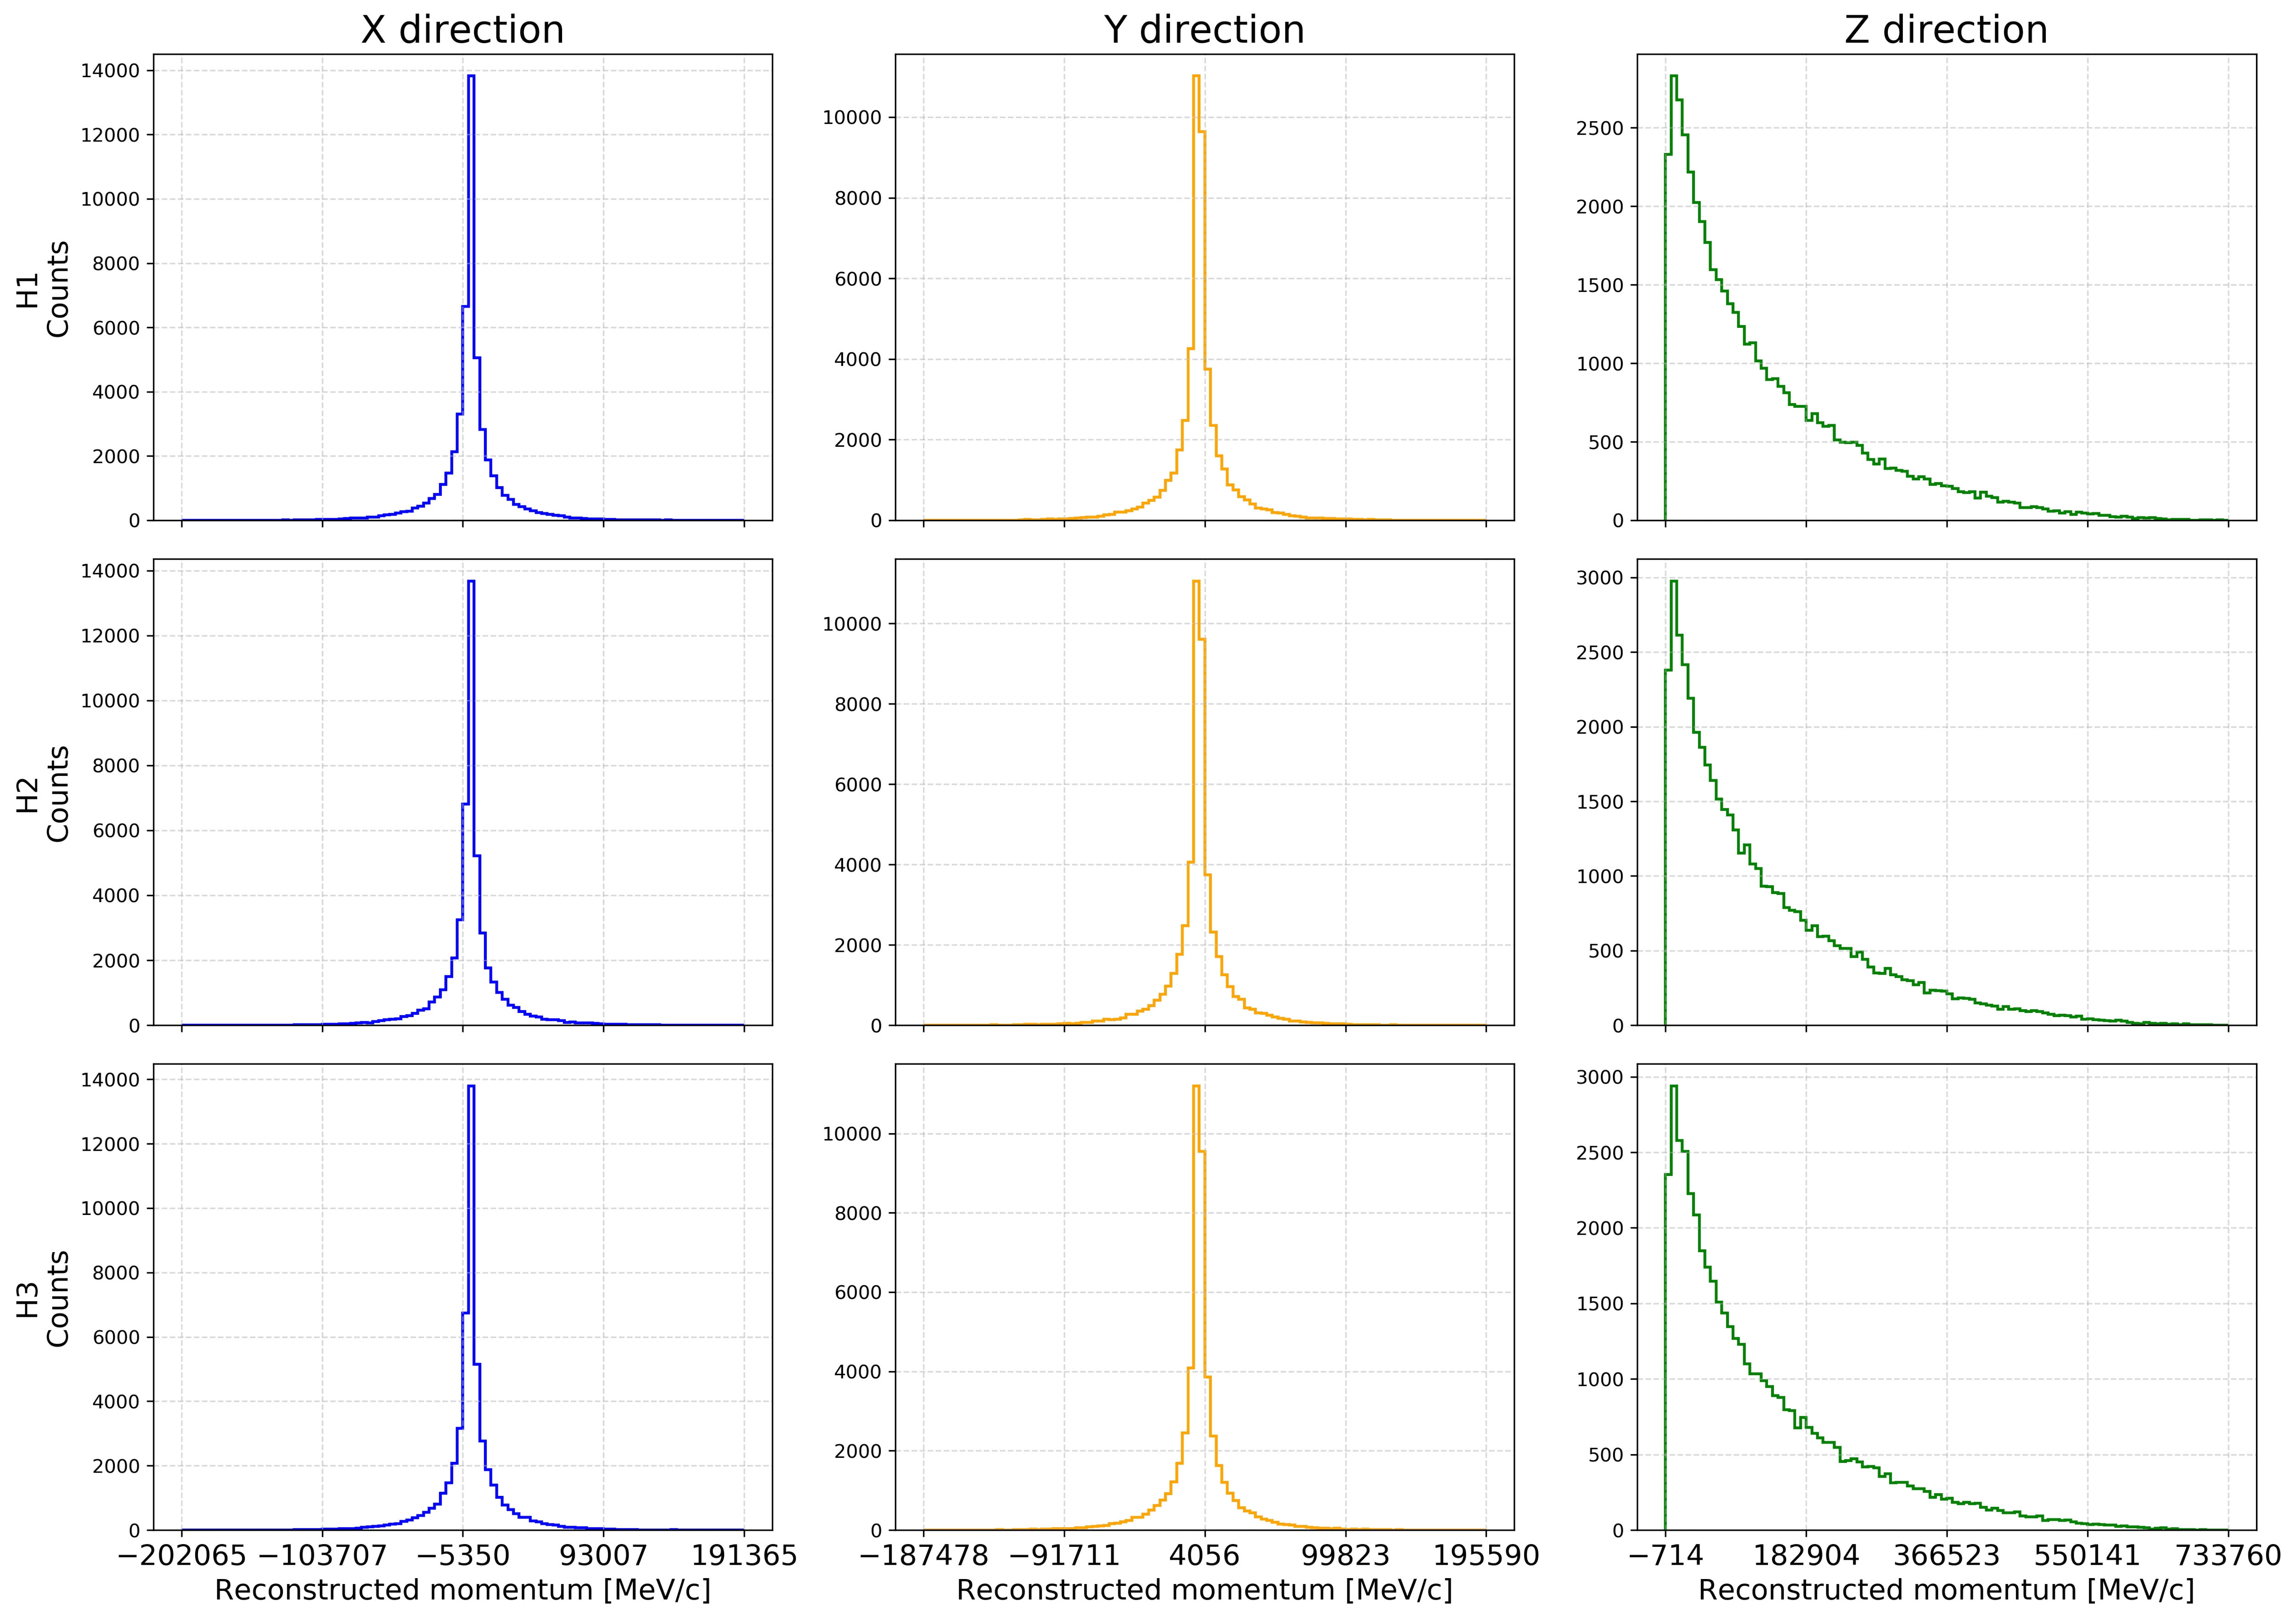
\includegraphics[scale=0.1]{Figure/hist_sim_p.png}
        \caption{Histogram of the momentum components of the three candidate kaons \(H_1\), \(H_2\), and \(H_3\). The \(x\)- and \(y\)-components are perpendicular to the beam \(z\)-axis.}
        \label{hist_sim_p}
    \end{figure}

    
    %% info for plot
    Thus, the simulation appears reasonable and the results provide a hint for further investigation in the experimental data.

    \begin{figure}[H]
        \centering
        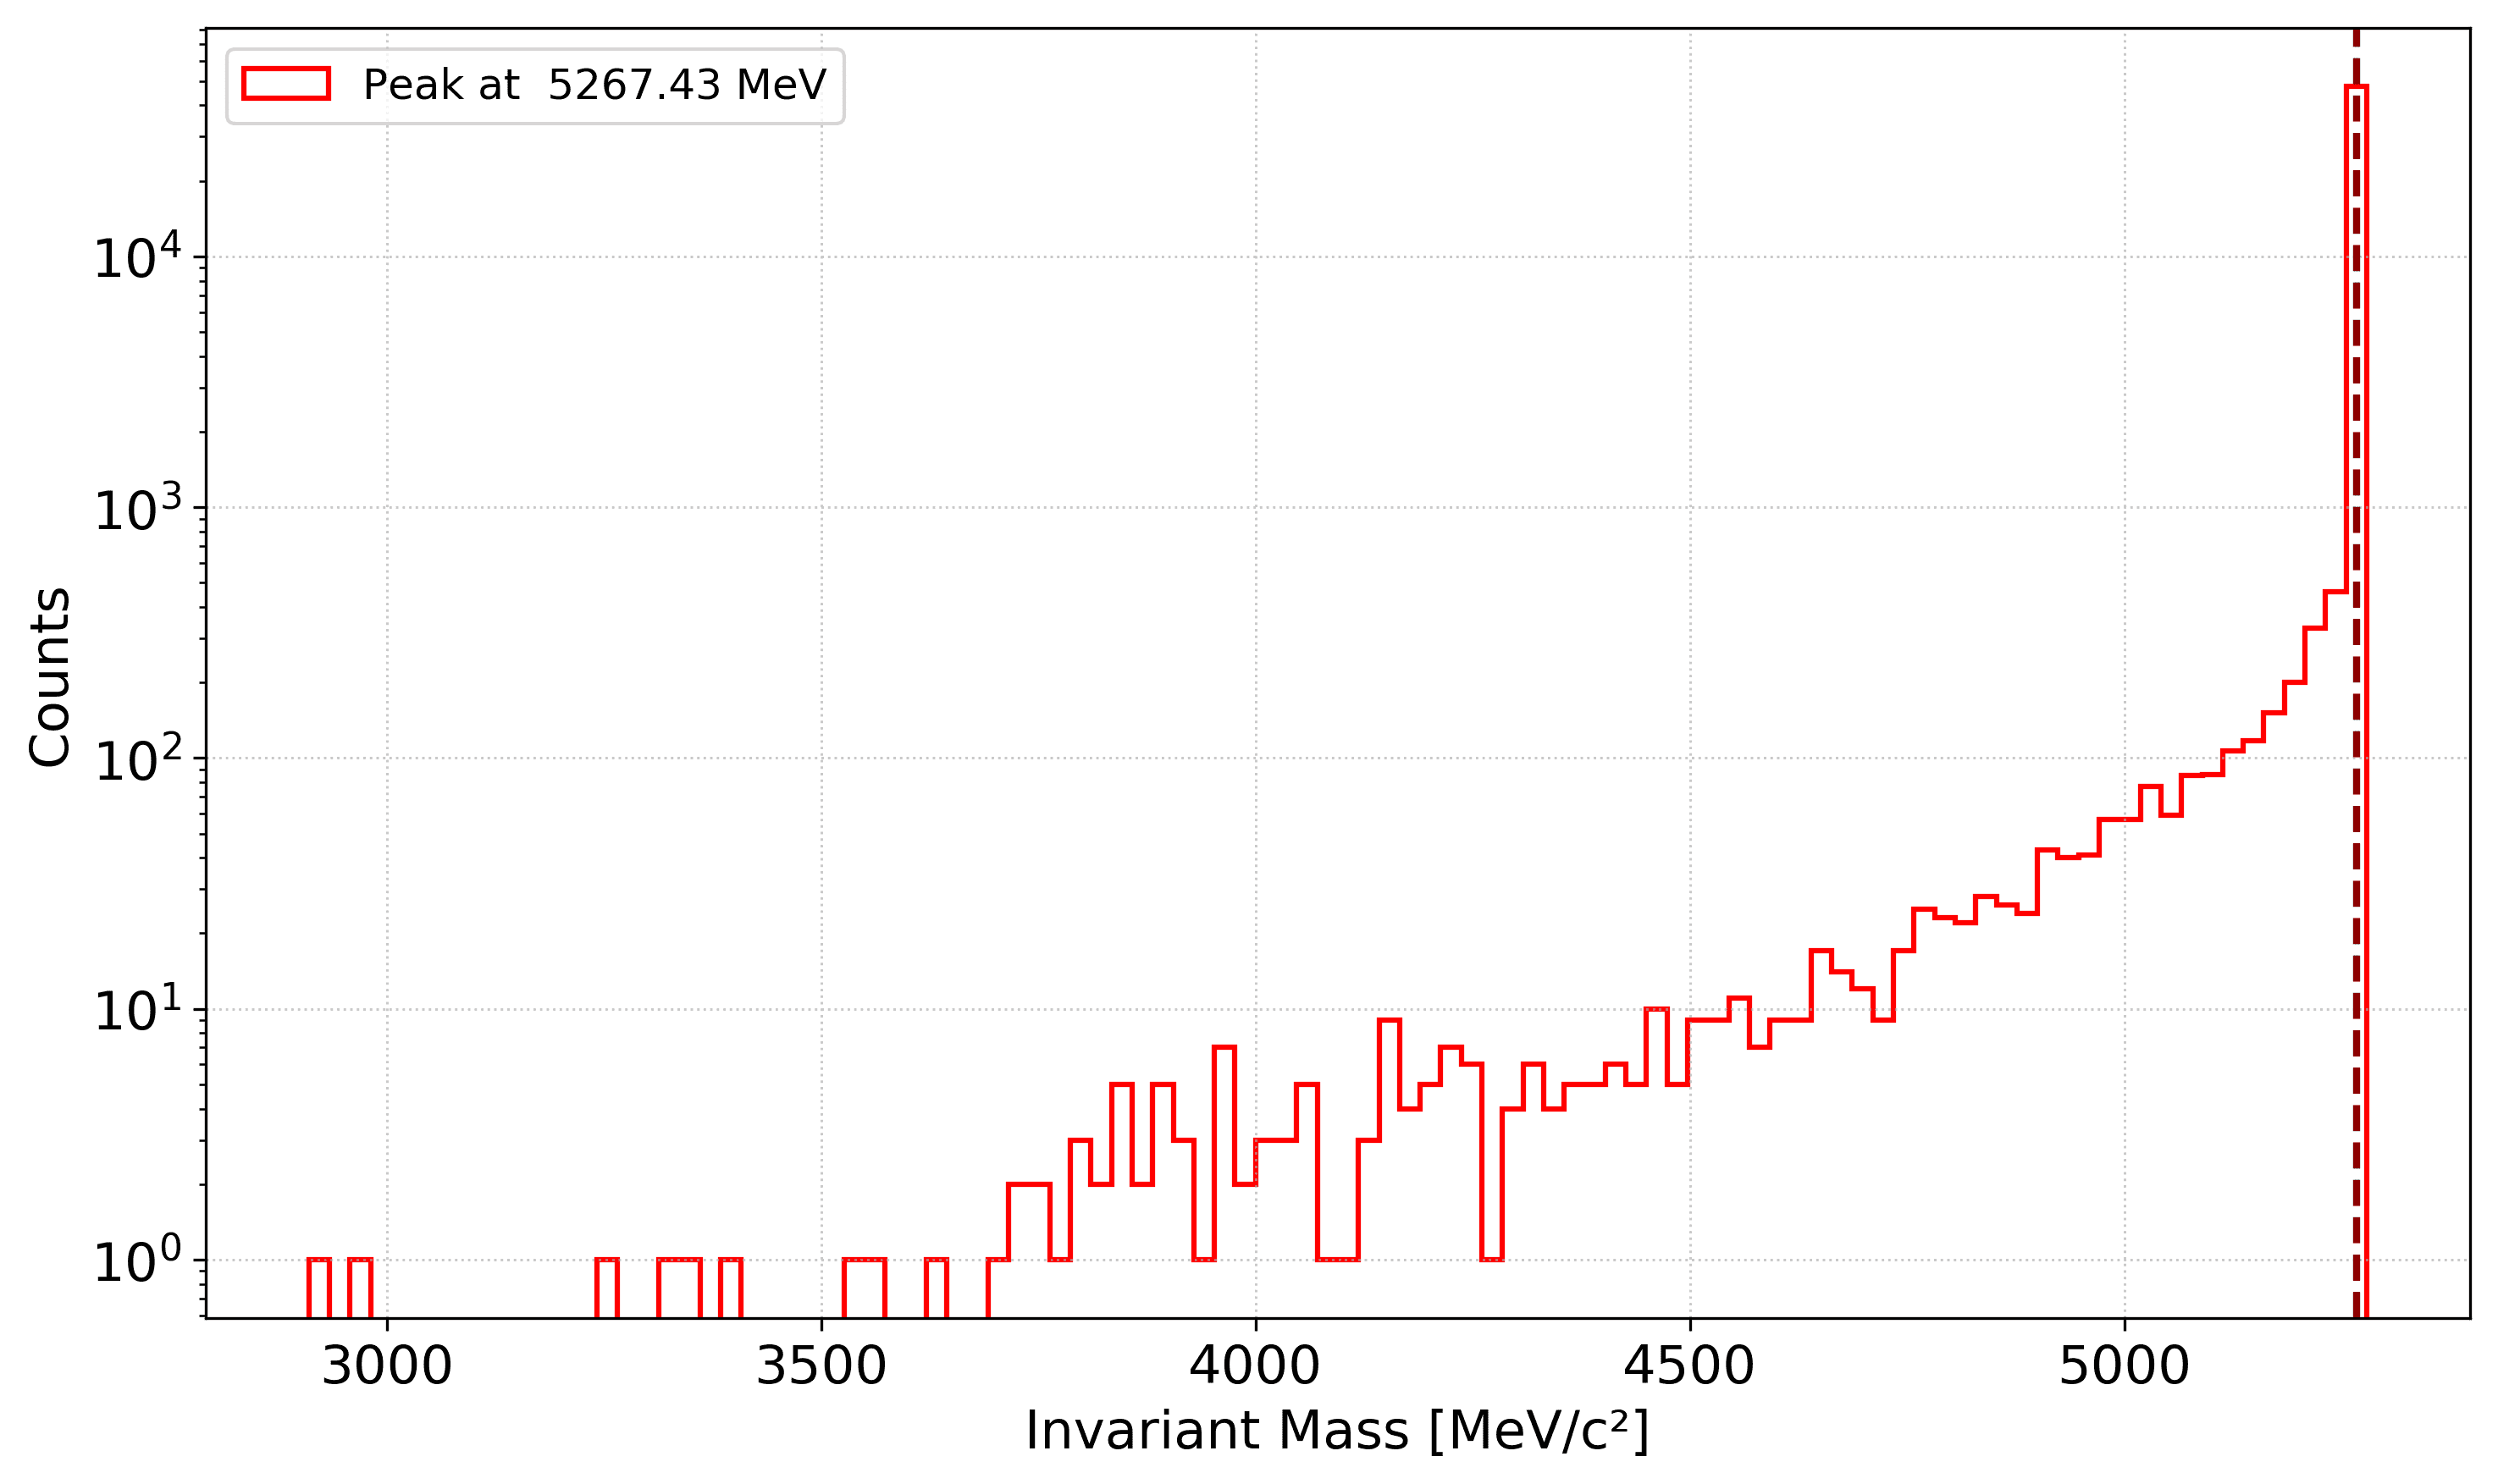
\includegraphics[scale=0.1]{Figure/hist_sim_mass.png}
        \caption{Histogram of the mass of \(B^\pm\) meson candidate.}
        \label{hist_sim_mass}
    \end{figure}
    \\
        
    \begin{figure}[H]
        \centering
        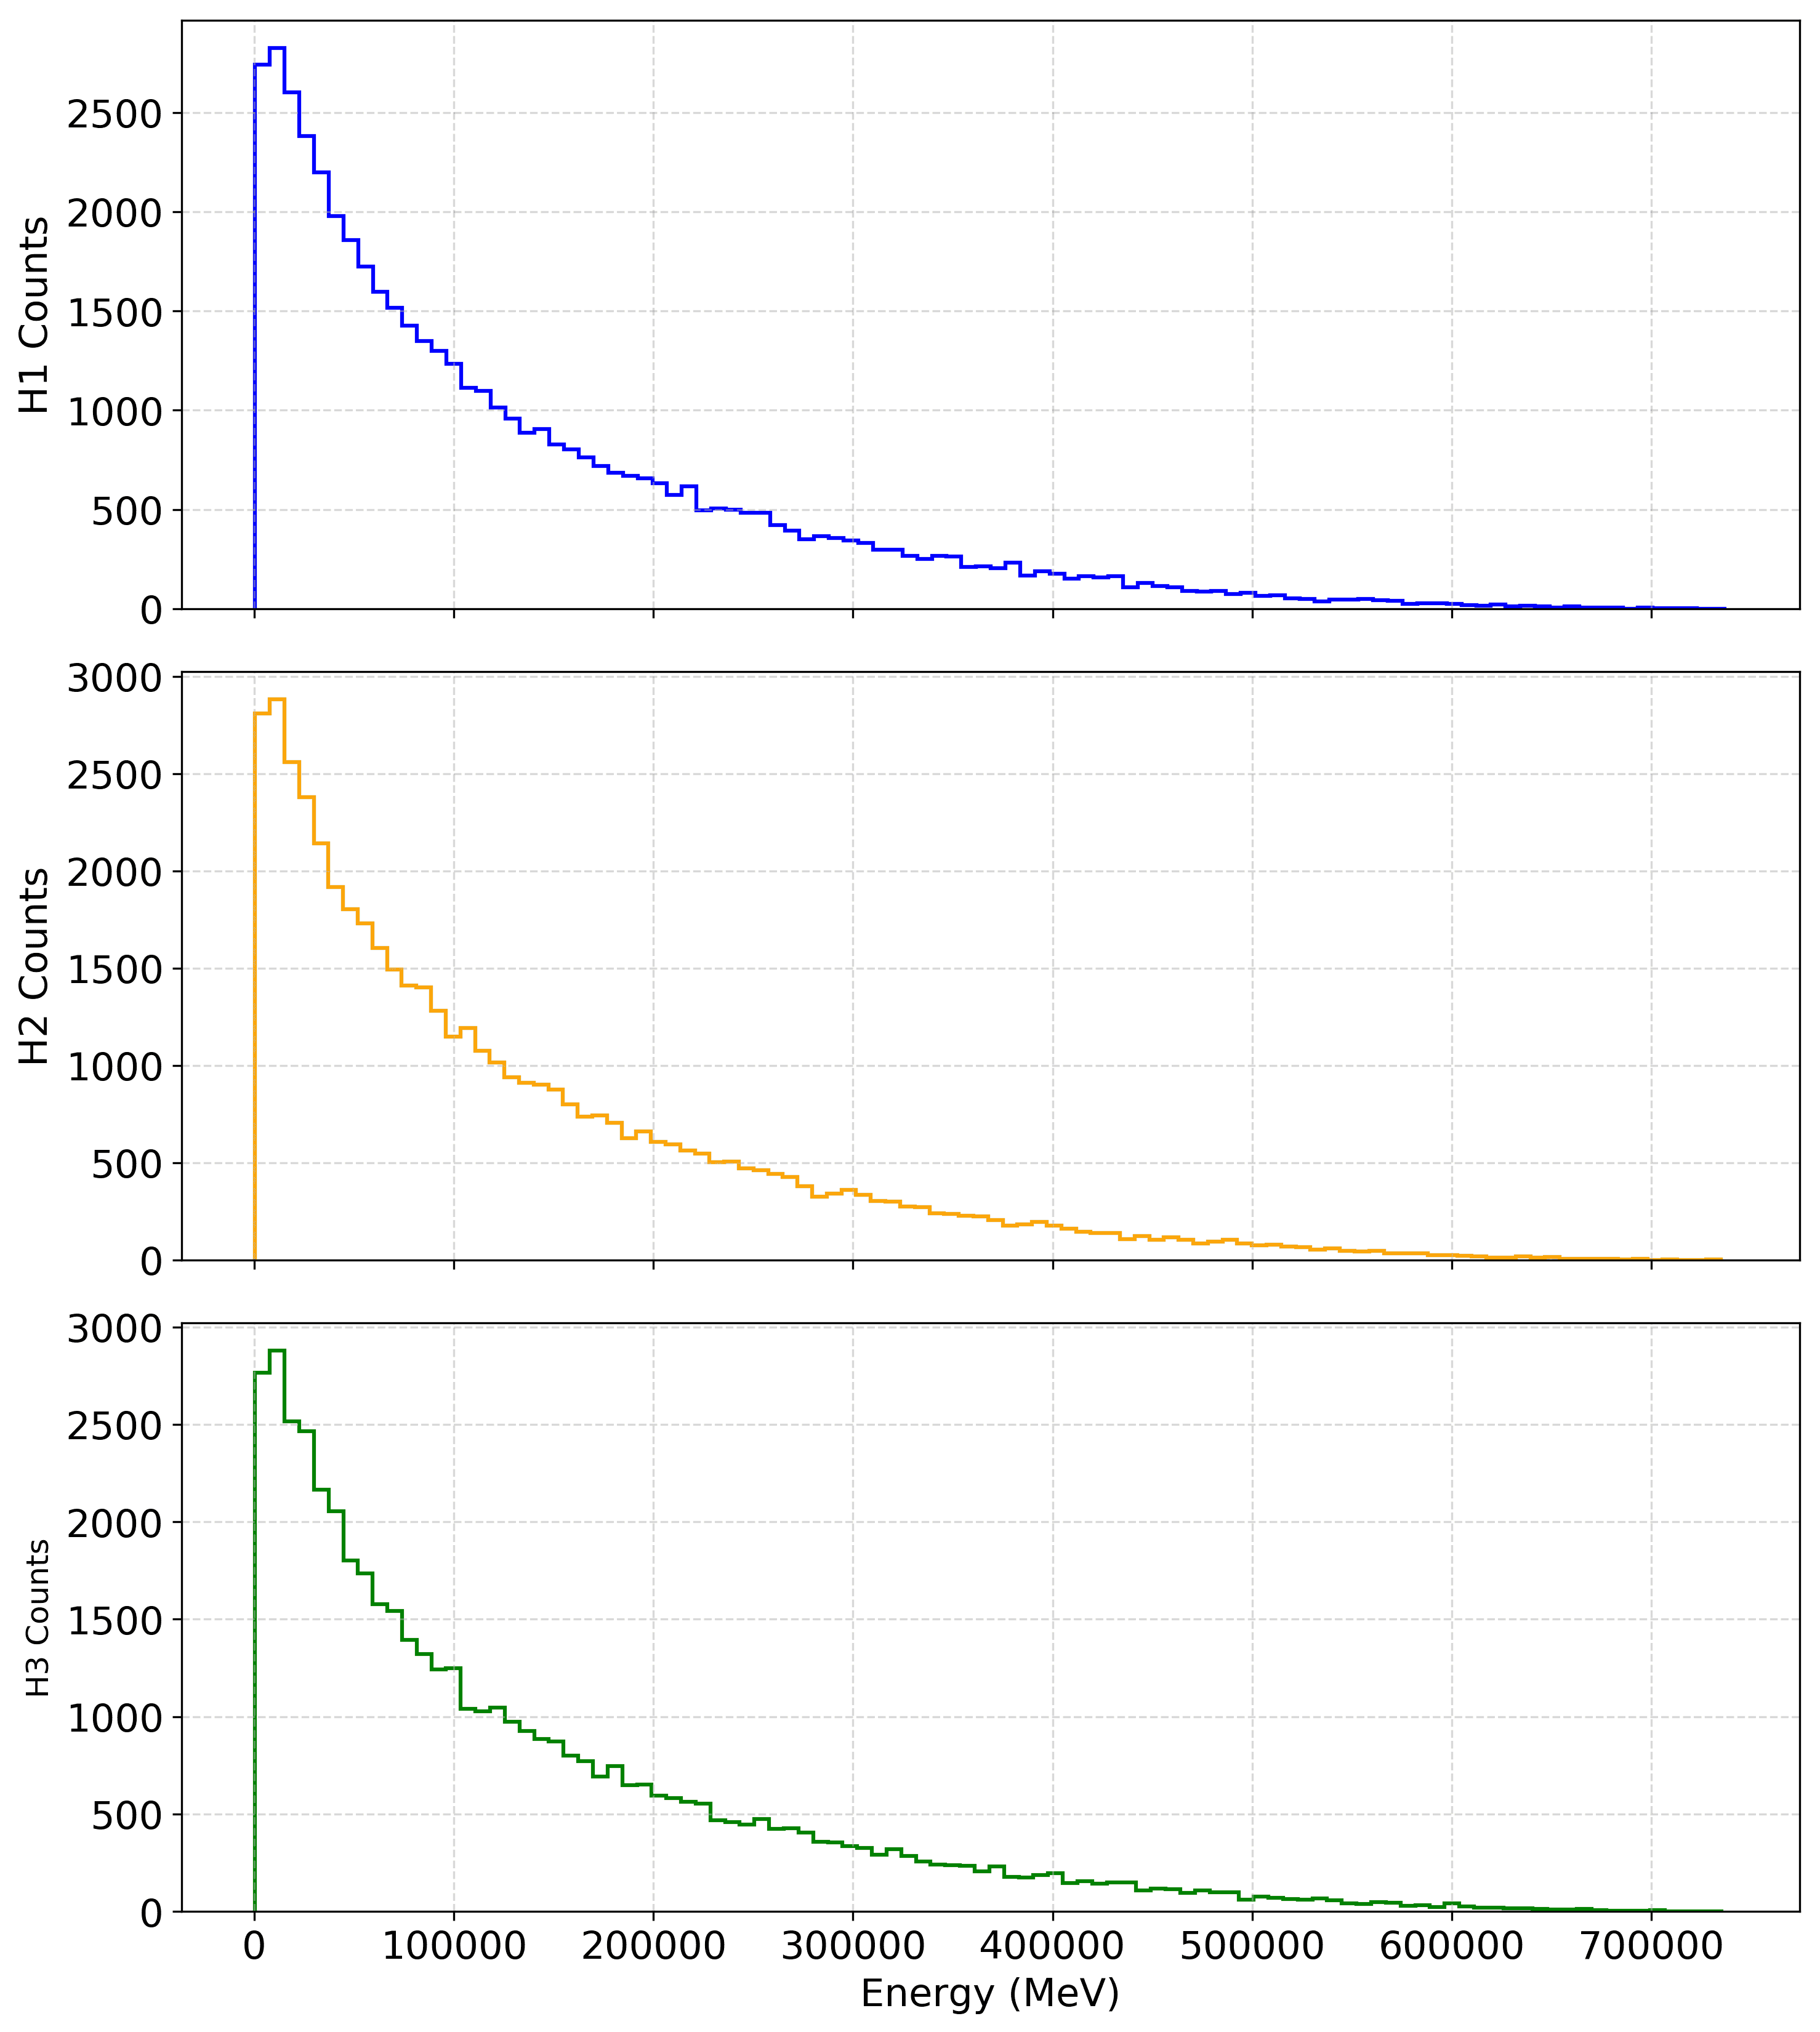
\includegraphics[scale=0.1]{Figure/hist_sim_energy.png}
        \caption{Histogram of the energy of the three candidate kaons.}
        \label{hist_sim_energy}
    \end{figure}
    \\
    
\section{\(B^+\) and  \(B^-\) decays from LHCb}

   To analyze LHCb experimental data, a preselection procedure is essential to reduce the combinatorial background and improve the signal-to-noise ratio. 
   This analysis was performed by applying the following criteria in Table \ref{table1}. Figure \ref{hist_prob} illustrates the probability distributions after applying the selection criteria.
   
    \begin{figure}[H]
        \centering
        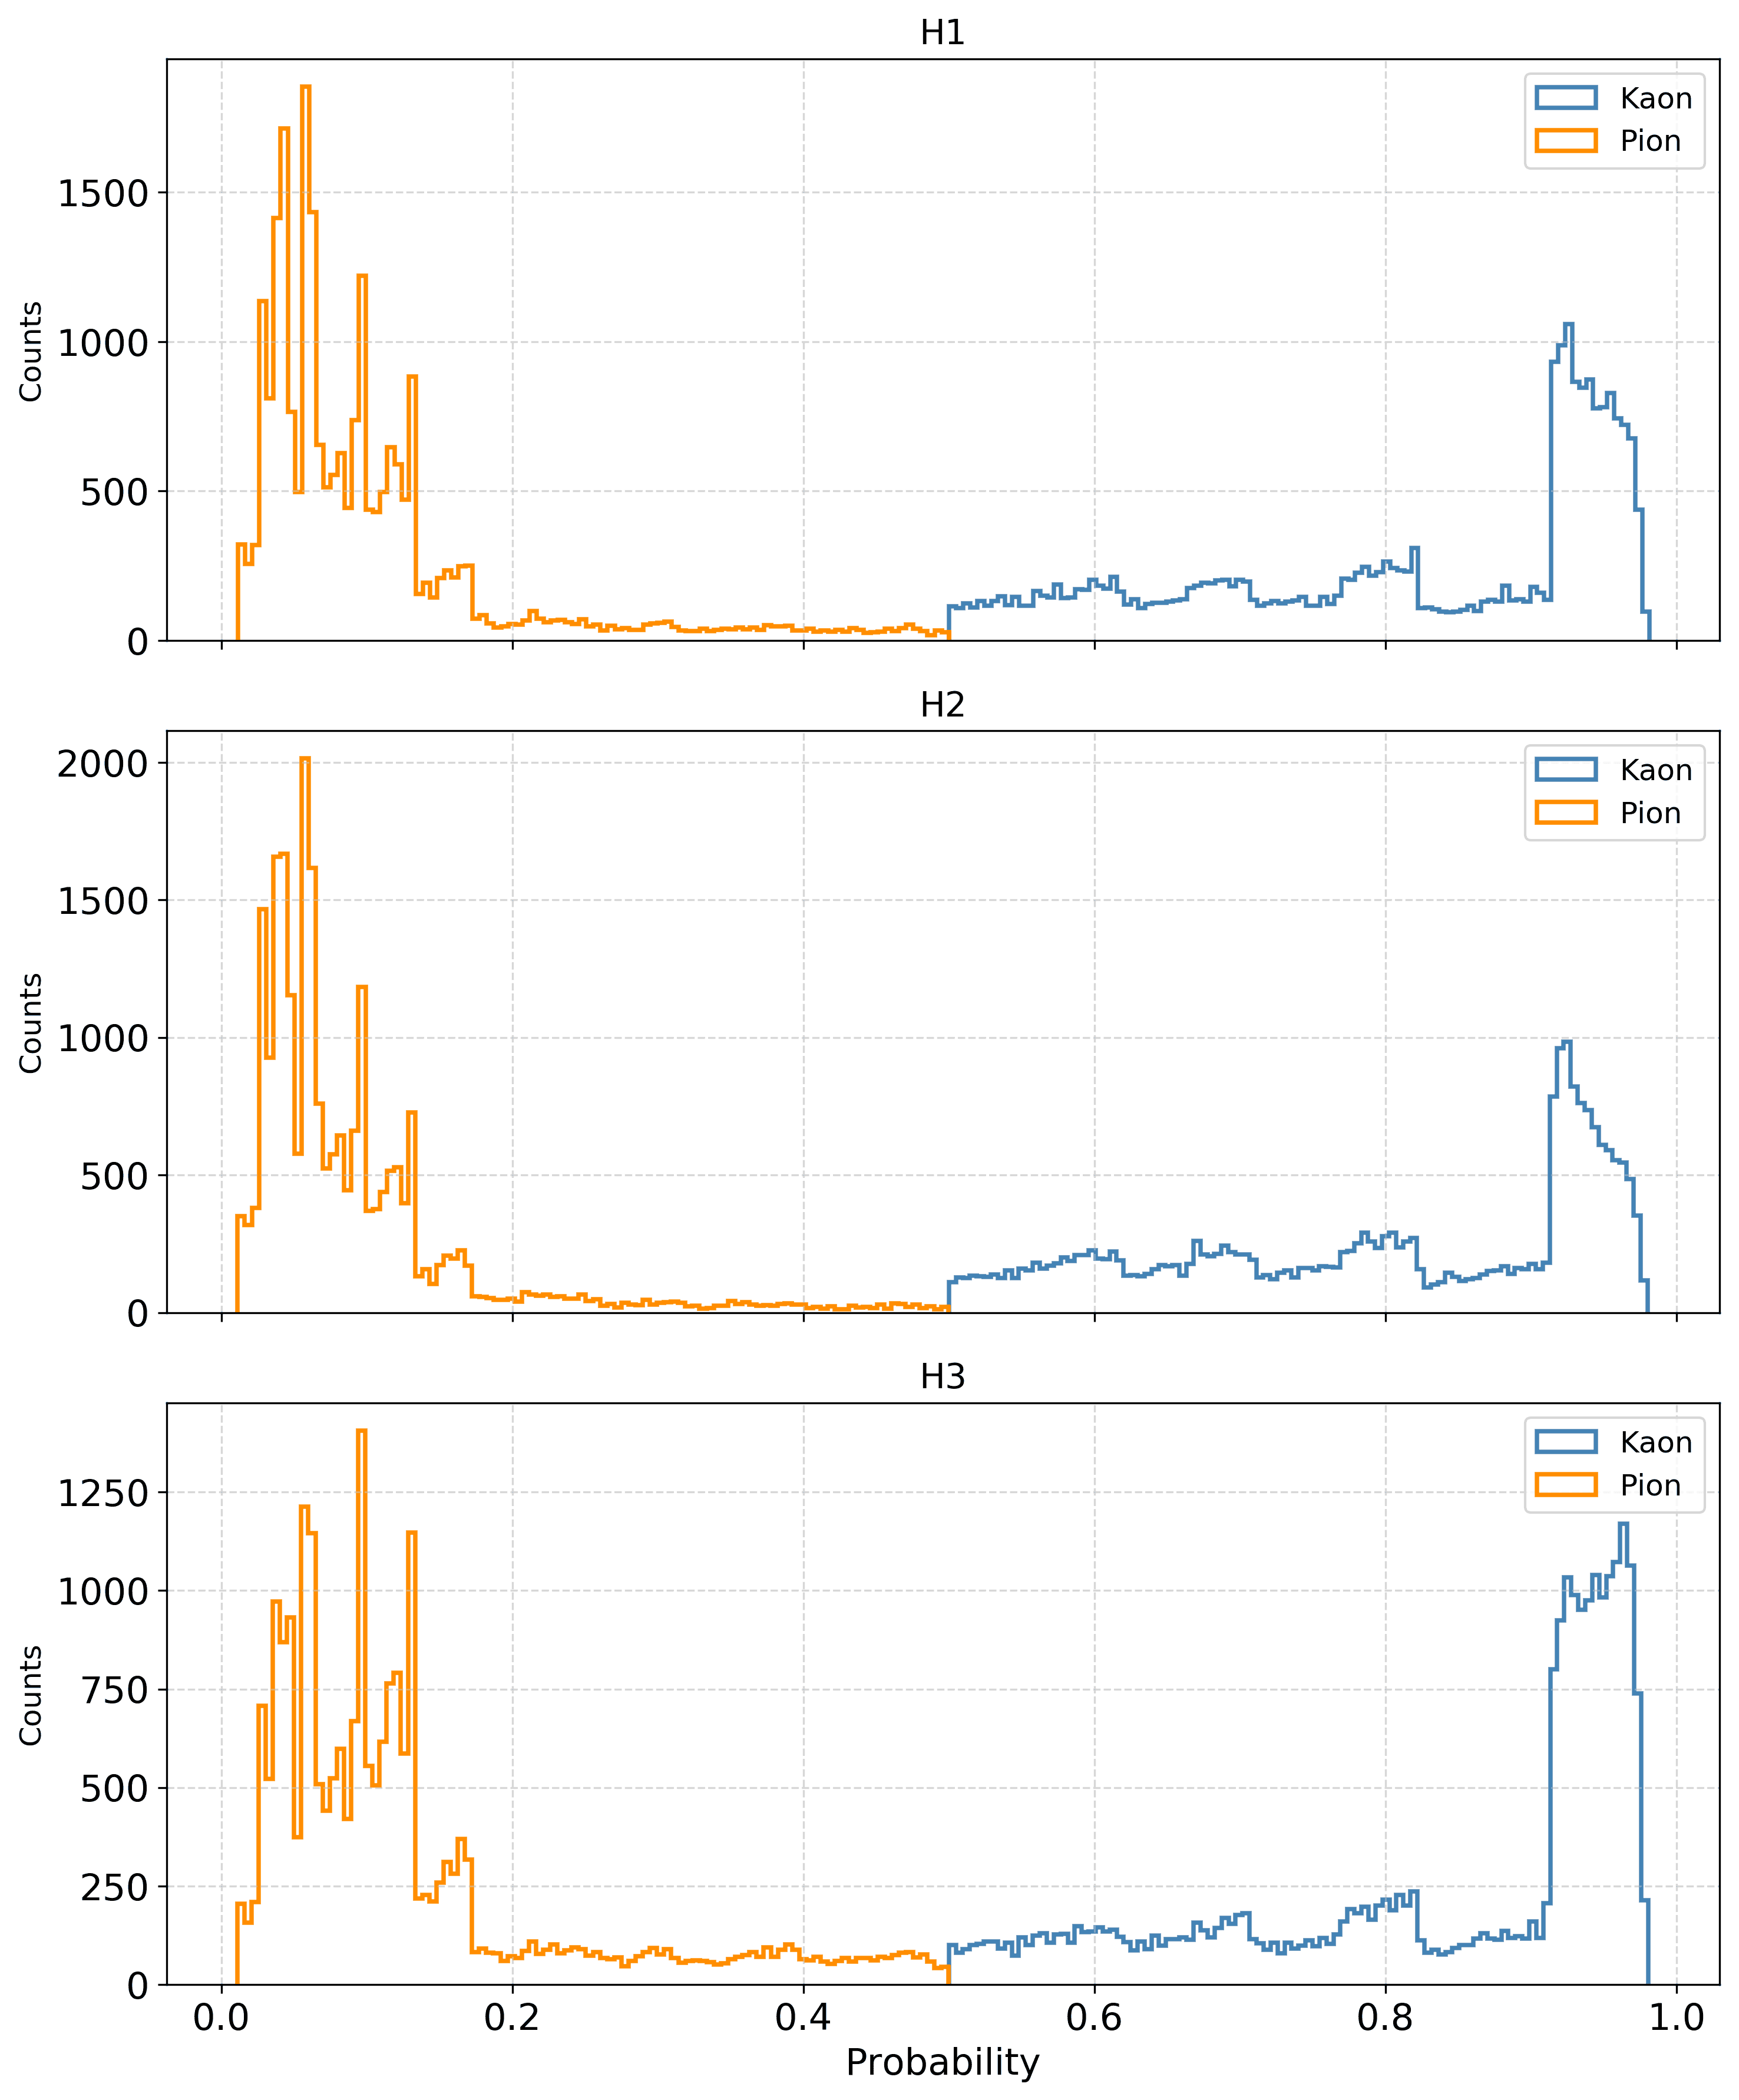
\includegraphics[scale=0.1]{Figure/hist_prob.png}
        \caption{Probability distribution of candidate kaons and Pions.}
        \label{hist_prob}
    \end{figure}

   The selection also ensures that muons are excluded. Following the procedure to calculate the mass of the \( B^\pm \) boson (see Equation \ref{eq_energy}), the results are shown in Figure \ref{hist_data_mass}. The mass peak at 5281.24 \(\text{MeV/$c^{2}$}\). compared to the simulated data peak at 5267.43 \(\text{MeV/$c^{2}$}\) is quite close and within reasonable agreement. The shape of the LHCb data clearly shows the challenges of measurement and simulation, including detector resolution effects and background contributions, as seen in Figure~\ref{hist_data_mass}.
   
    \begin{table}
    \centering
    \caption{Preselection criteria applied to candidate kaons in the analysis.}
    \label{tab:preselection_criteria}
    \begin{tabular}{lccc}
    \hline
    \textbf{Criterion} & \textbf{H1} & \textbf{H2} & 
    \textbf{H3} \\
    \hline
    isMuon & $0$ & $0$ & $0$
    \\[6pt]
    Probability of being a pion & $< 0.5$ & $< 0.5$ & $< 0.5$ \\[6pt]
    Probability of being a kaon & $> 0.5$ & $> 0.5$ & $> 0.5$ \\
    \hline
    \label{table1}
    \end{tabular}
    \end{table}  
    \\
    
    % %% info for plot
    %     The mass distribution of the \(B^\pm\) meson candidates is shown in Figure \ref{hist_sim_mass}. The peak of the histogram is at 5267.43 MeV.


 
    \begin{figure}[H]
        \centering
        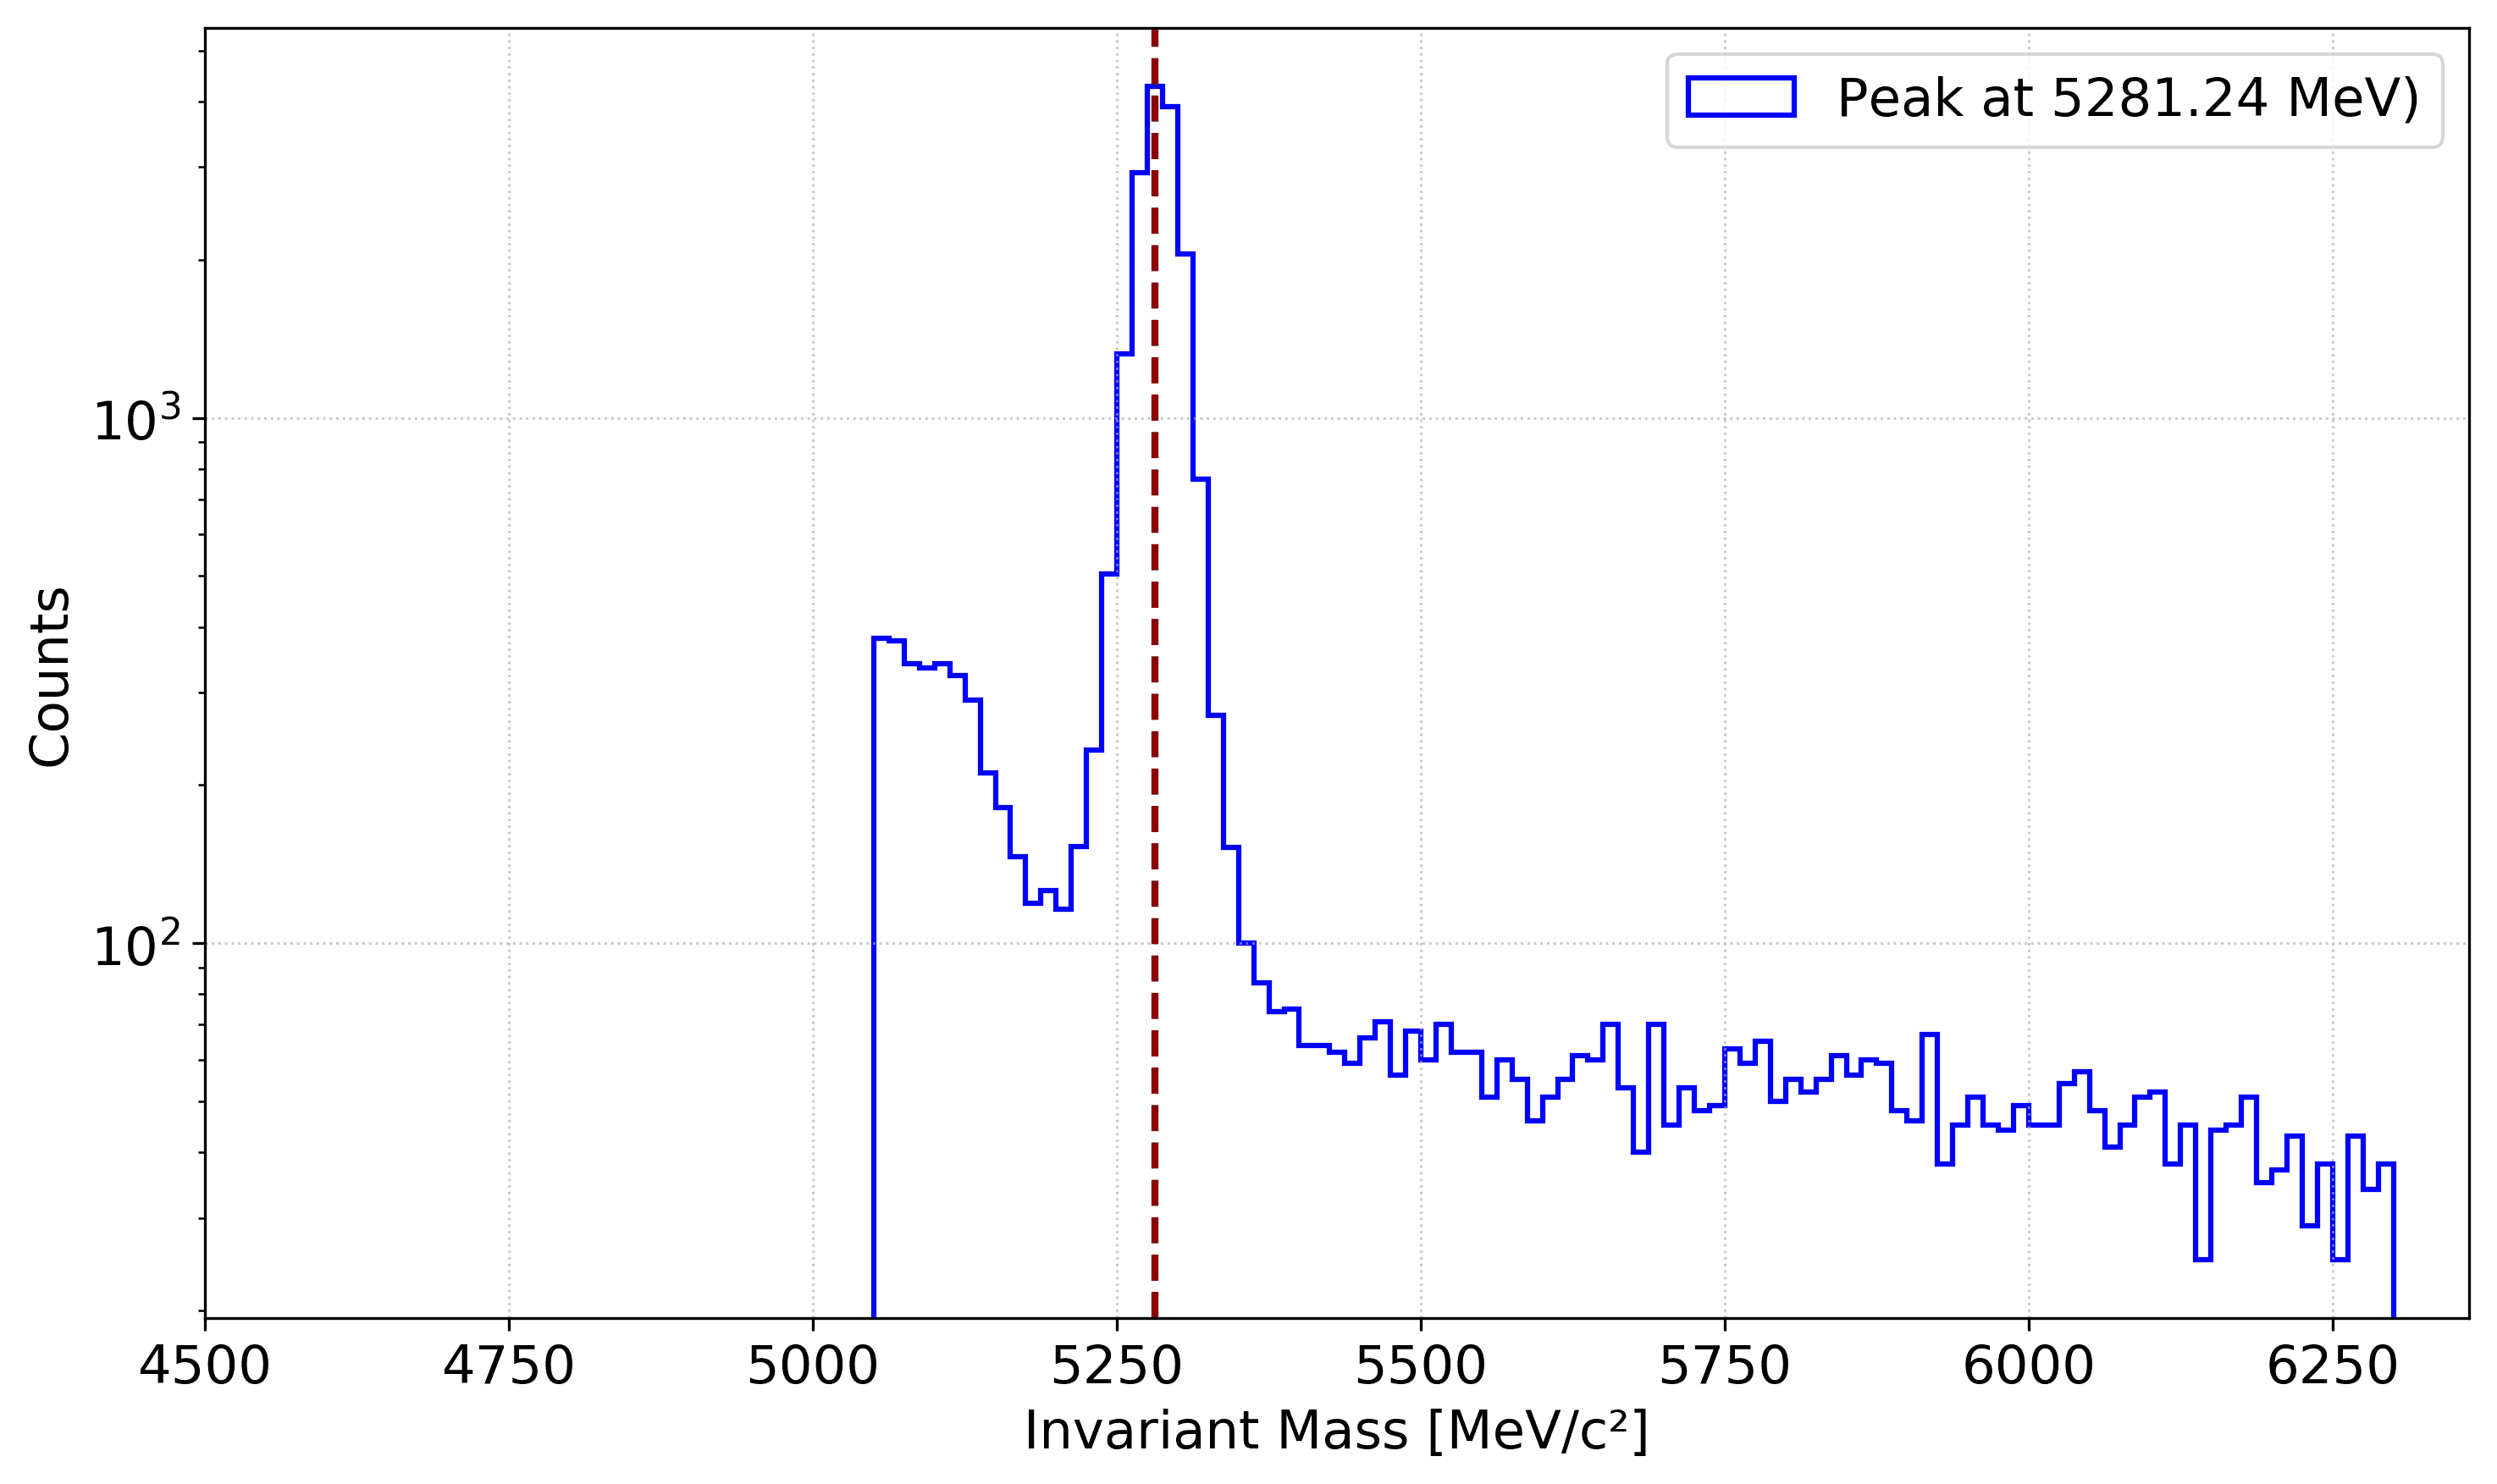
\includegraphics[scale=0.1]{Figure/hist_data_mass.png}
        \caption{Histogram of the mass of \(B^\pm\) meson candidate from LHCb experiment.}
        \label{hist_data_mass}
    \end{figure}
    \\

    \section{Global CP violation}
    \label{sec:global_asymmetry}
    To investigate CP violation, the \(B^\pm\) meson candidates are separated based on the charge conservation of the three kaon candidate decay products, \(B^+ \to K^+ K^+ K^-\) and \(B^- \to K^- K^- K^+\). To search for global matter–antimatter asymmetry, the following equation is used to determine the asymmetry:
    
    \begin{equation}
    A = \frac{N^+ - N^-}{N^+ + N^-}
    \label{asym}
    \end{equation}

    where \(N^+\) and \(N^-\) represent the number of \(B^+\) and \(B^-\) candidates, respectively.
    \\
    
    However, the observed asymmetry may not arise from CP violation. It can also include contributions from other sources such as production asymmetry, where the initial number of produced \(B^+\) and \(B^-\) mesons differs due to proton–proton collision dynamics and detection asymmetry, where the detector may have different efficiencies for positively and negatively charged particles. These effects must be  considered and corrected in order to isolate the true CP-violating asymmetry.
    \\
    
    The statistical uncertainty of the asymmetry can be calculated using the formula:

    \begin{equation}
    \sigma_A = \sqrt{\frac{1 - A^2}{N^+ + N^-}}
    \label{sigma}
    \end{equation}

    \\ 
    
    where \(A\) is the true asymmetry, and \(N^+\) and \(N^-\) are the numbers of \(B^+\) and \(B^-\) meson candidates, respectively.
    \\  
    
    More importantly, in particle physics, the significance of the result is based on the ratio of the measured asymmetry to its statistical uncertainty \(\sigma_A\). This significance indicates how likely it is that the observed asymmetry is not due to random fluctuations.

    \begin{equation}
    \text{Significance} = \frac{A}{\sigma_A}
    \label{sig}
    \end{equation}

    The table below shows the results obtained in this analysis.

    \begin{table}[H]
    \centering
    \begin{tabular}{lccc}
        \hline
        \textbf{Observable} & \textbf{Value} & \textbf{Uncertainty \(\sigma_A\)} & \textbf{Significance \(\frac{A}{\sigma_A}\)} \\
        \hline
        Asymmetry \(A_{global}\) & 0.0370 & 0.0065 & 5.7291 \\
        \hline
    \end{tabular}
    \caption{Summary of the global CP asymmetry.}
    \label{asymmetry-results}
    \end{table}
    
    According to standard conventions, a significance greater than \(5\sigma\) is considered a discovery. It is evident that the result in this analysis confirms the discovery of CP violation.
    \\

    \section{Local CP violation}
    To further investigate CP violation, local CP asymmetries are explored by analyzing the Dalitz plot distribution of the decay products by the calculation of the invariant masses of the hadron pairs \( H1\,H2 \) and \( H1\, H3 \). This method is  useful for identifying resonances in the two-body subsystems of the three-body decay. 
    \\ 
    
    Figure \ref{dalitz_data}(a) shows the scatter plot comparing Simulation and LHCb data. It is clear that there are regions with a higher density of points in the data whereas the simulation displays a more uniform distribution within the triangular phase space. This occurs because the decay of the \(B\) meson can also proceed via an intermediate resonance. The decay \(B^+ \to K^+ K^+ K^-\) may proceed through the channel \(B^+ \to K^+ R^0\). Decays involving \( R^0 \) have different CP-violation effects as this is effectively a quasi two-body decay. For simplicity, the \( R^0 \to K^+ K^- \) channel is excluded.
    \\
    
     To extract detailed information, The Dalitz plot analysis can be further impose an ordering on these resonances based on their invariant masses. The resonance with the higher mass is labeled \( R^0_{\text{High}} \) and the one with the lower mass is labeled \( R^0_{\text{Low}} \). This sorting allows for clearer separation and better interpretation of the resonance structures in the Dalitz plot as shown the Figure \ref{dalitz_data}(b).
     \\

    Figure \ref{dalitz_data} identifies resonances in the two-body subsystems in two different regions: one around \(3.48 \times 10^6\,\mathrm{MeV}^2/c^4\) and another around \(11.7 \times 10^6\,\mathrm{MeV}^2/c^4\). These regions correspond to the masses of the \(D^0\) meson (\(\sim 1865\,\mathrm{MeV}/c^2\)) and the \(\chi_{c0}\) meson (\(\sim 3415\,\mathrm{MeV}/c^2\)).

    
    \begin{figure}[H]
        \centering
        \begin{subfigure}[b]{0.48\textwidth}
            \centering
            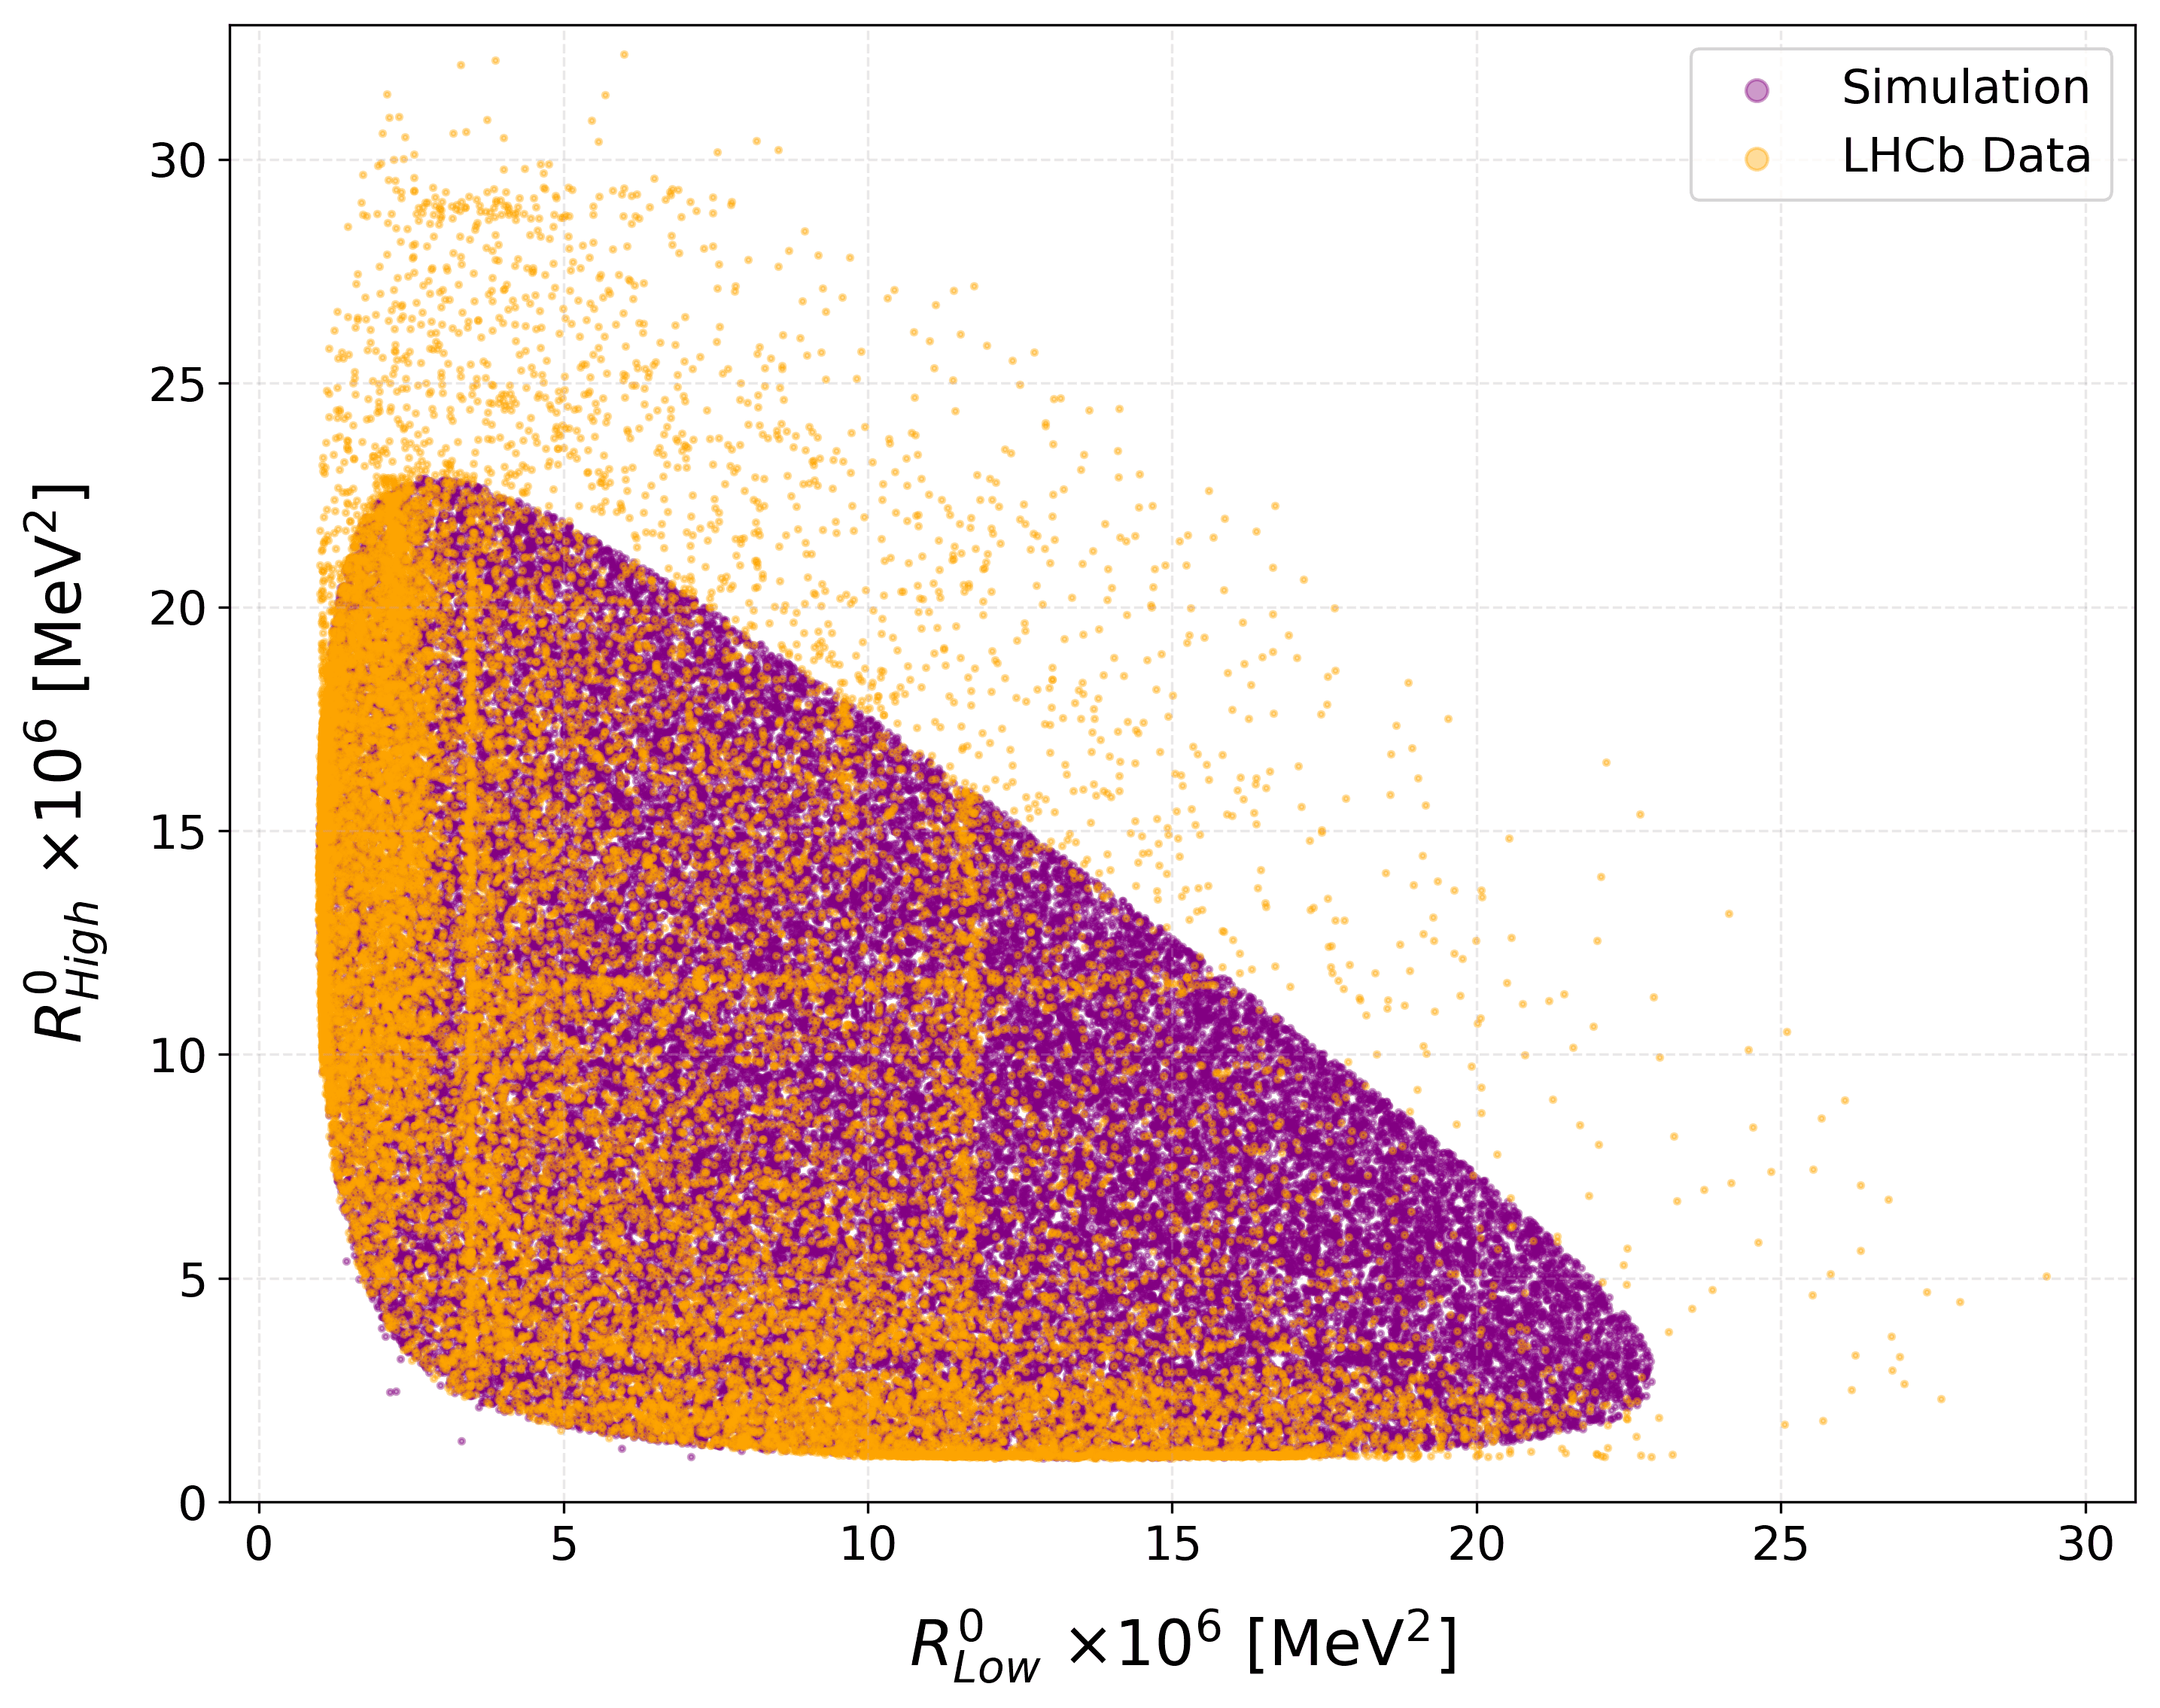
\includegraphics[width=\textwidth, scale=0.35]{Figure/dalitz_data_sim.png}
            \caption{Scatter plot comparing the Simulation and LHCb data distributions}
        \end{subfigure}
        \hfill
        \begin{subfigure}[b]{0.48\textwidth}
            \centering
            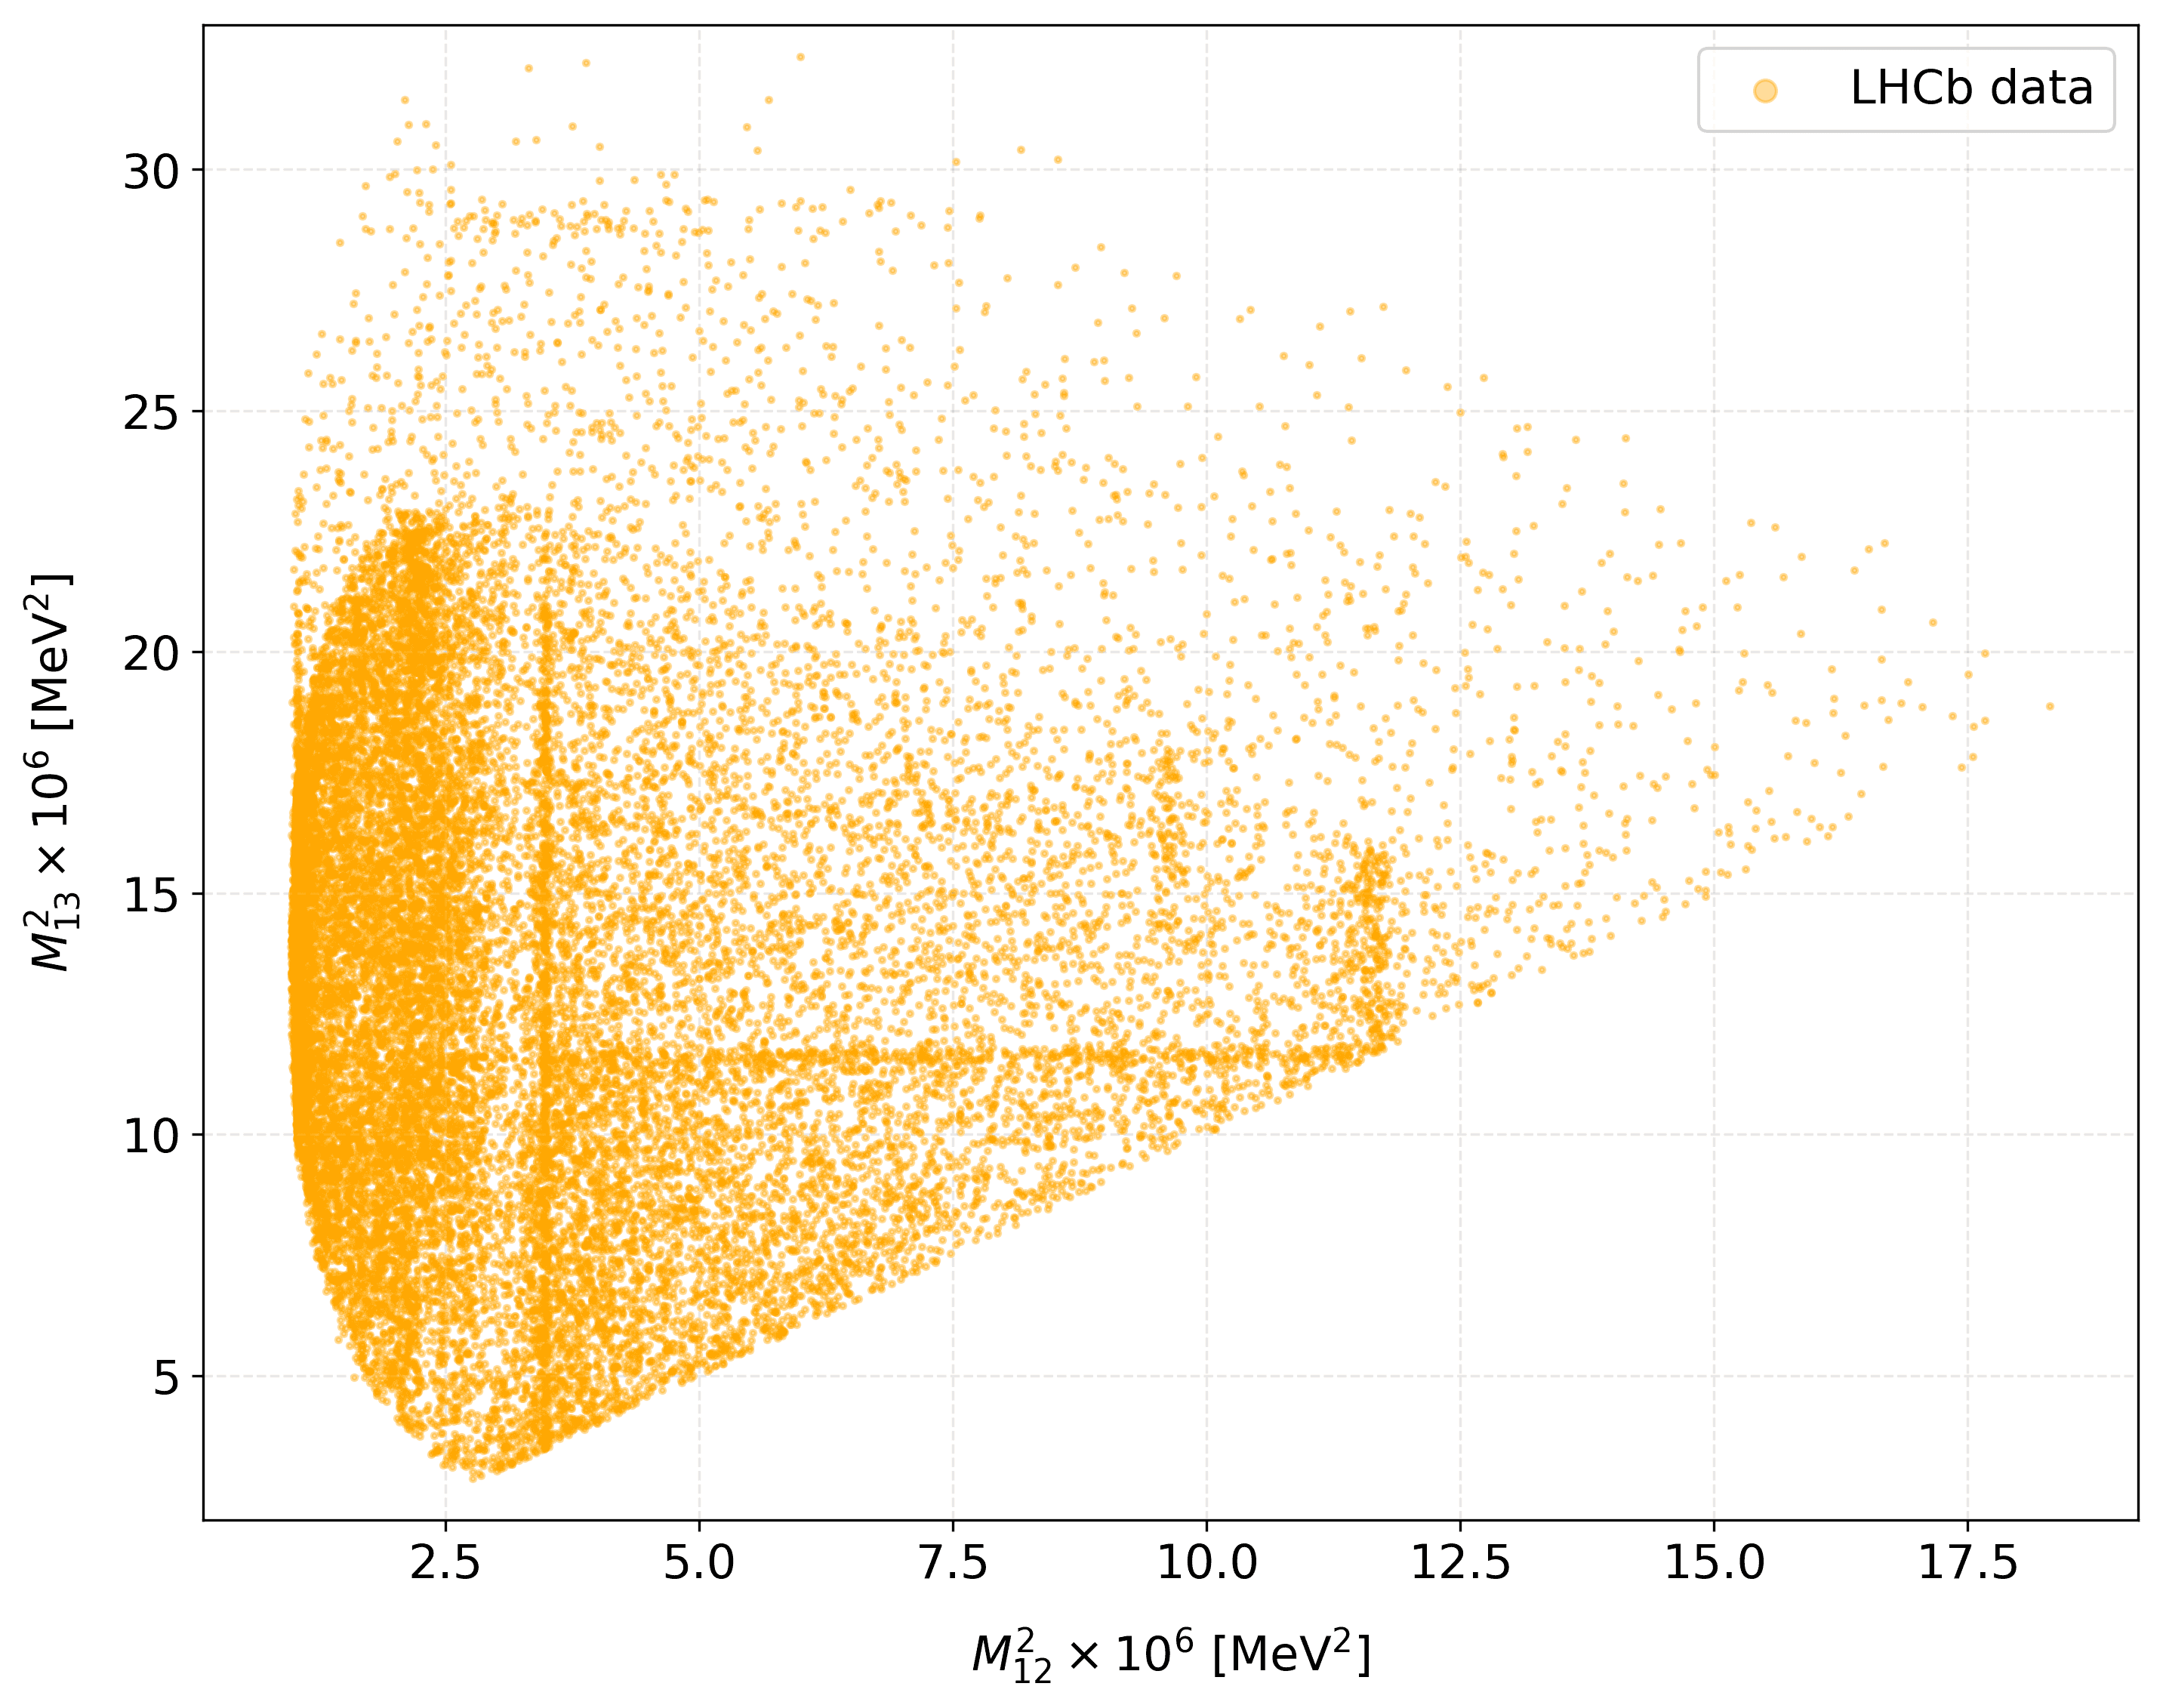
\includegraphics[width=\textwidth, scale=0.35]{Figure/dalitz_data_ordering.png}
           \caption{Ordering of the resonances High and Low based on the invariant mass}
        \end{subfigure}
        \caption{Dalitz plot distribution of the decay products.}
        \label{dalitz_data}
    \end{figure}
    \\

    To ensure a more precise analysis, the regions corresponding to the \(D^0\) meson and the \(\chi_{c0}\) meson will be excluded from the subsequent analysis. Figure \ref{hist_dalitz_data_cut} shows the Dalitz plot before and after excluding the regions corresponding to the \(D^0\) and \(\chi_{c0}\) mesons.

    %% why there is red at  00
 

    \begin{figure}[H]
        \centering
        \begin{subfigure}[b]{0.48\textwidth}
            \centering
            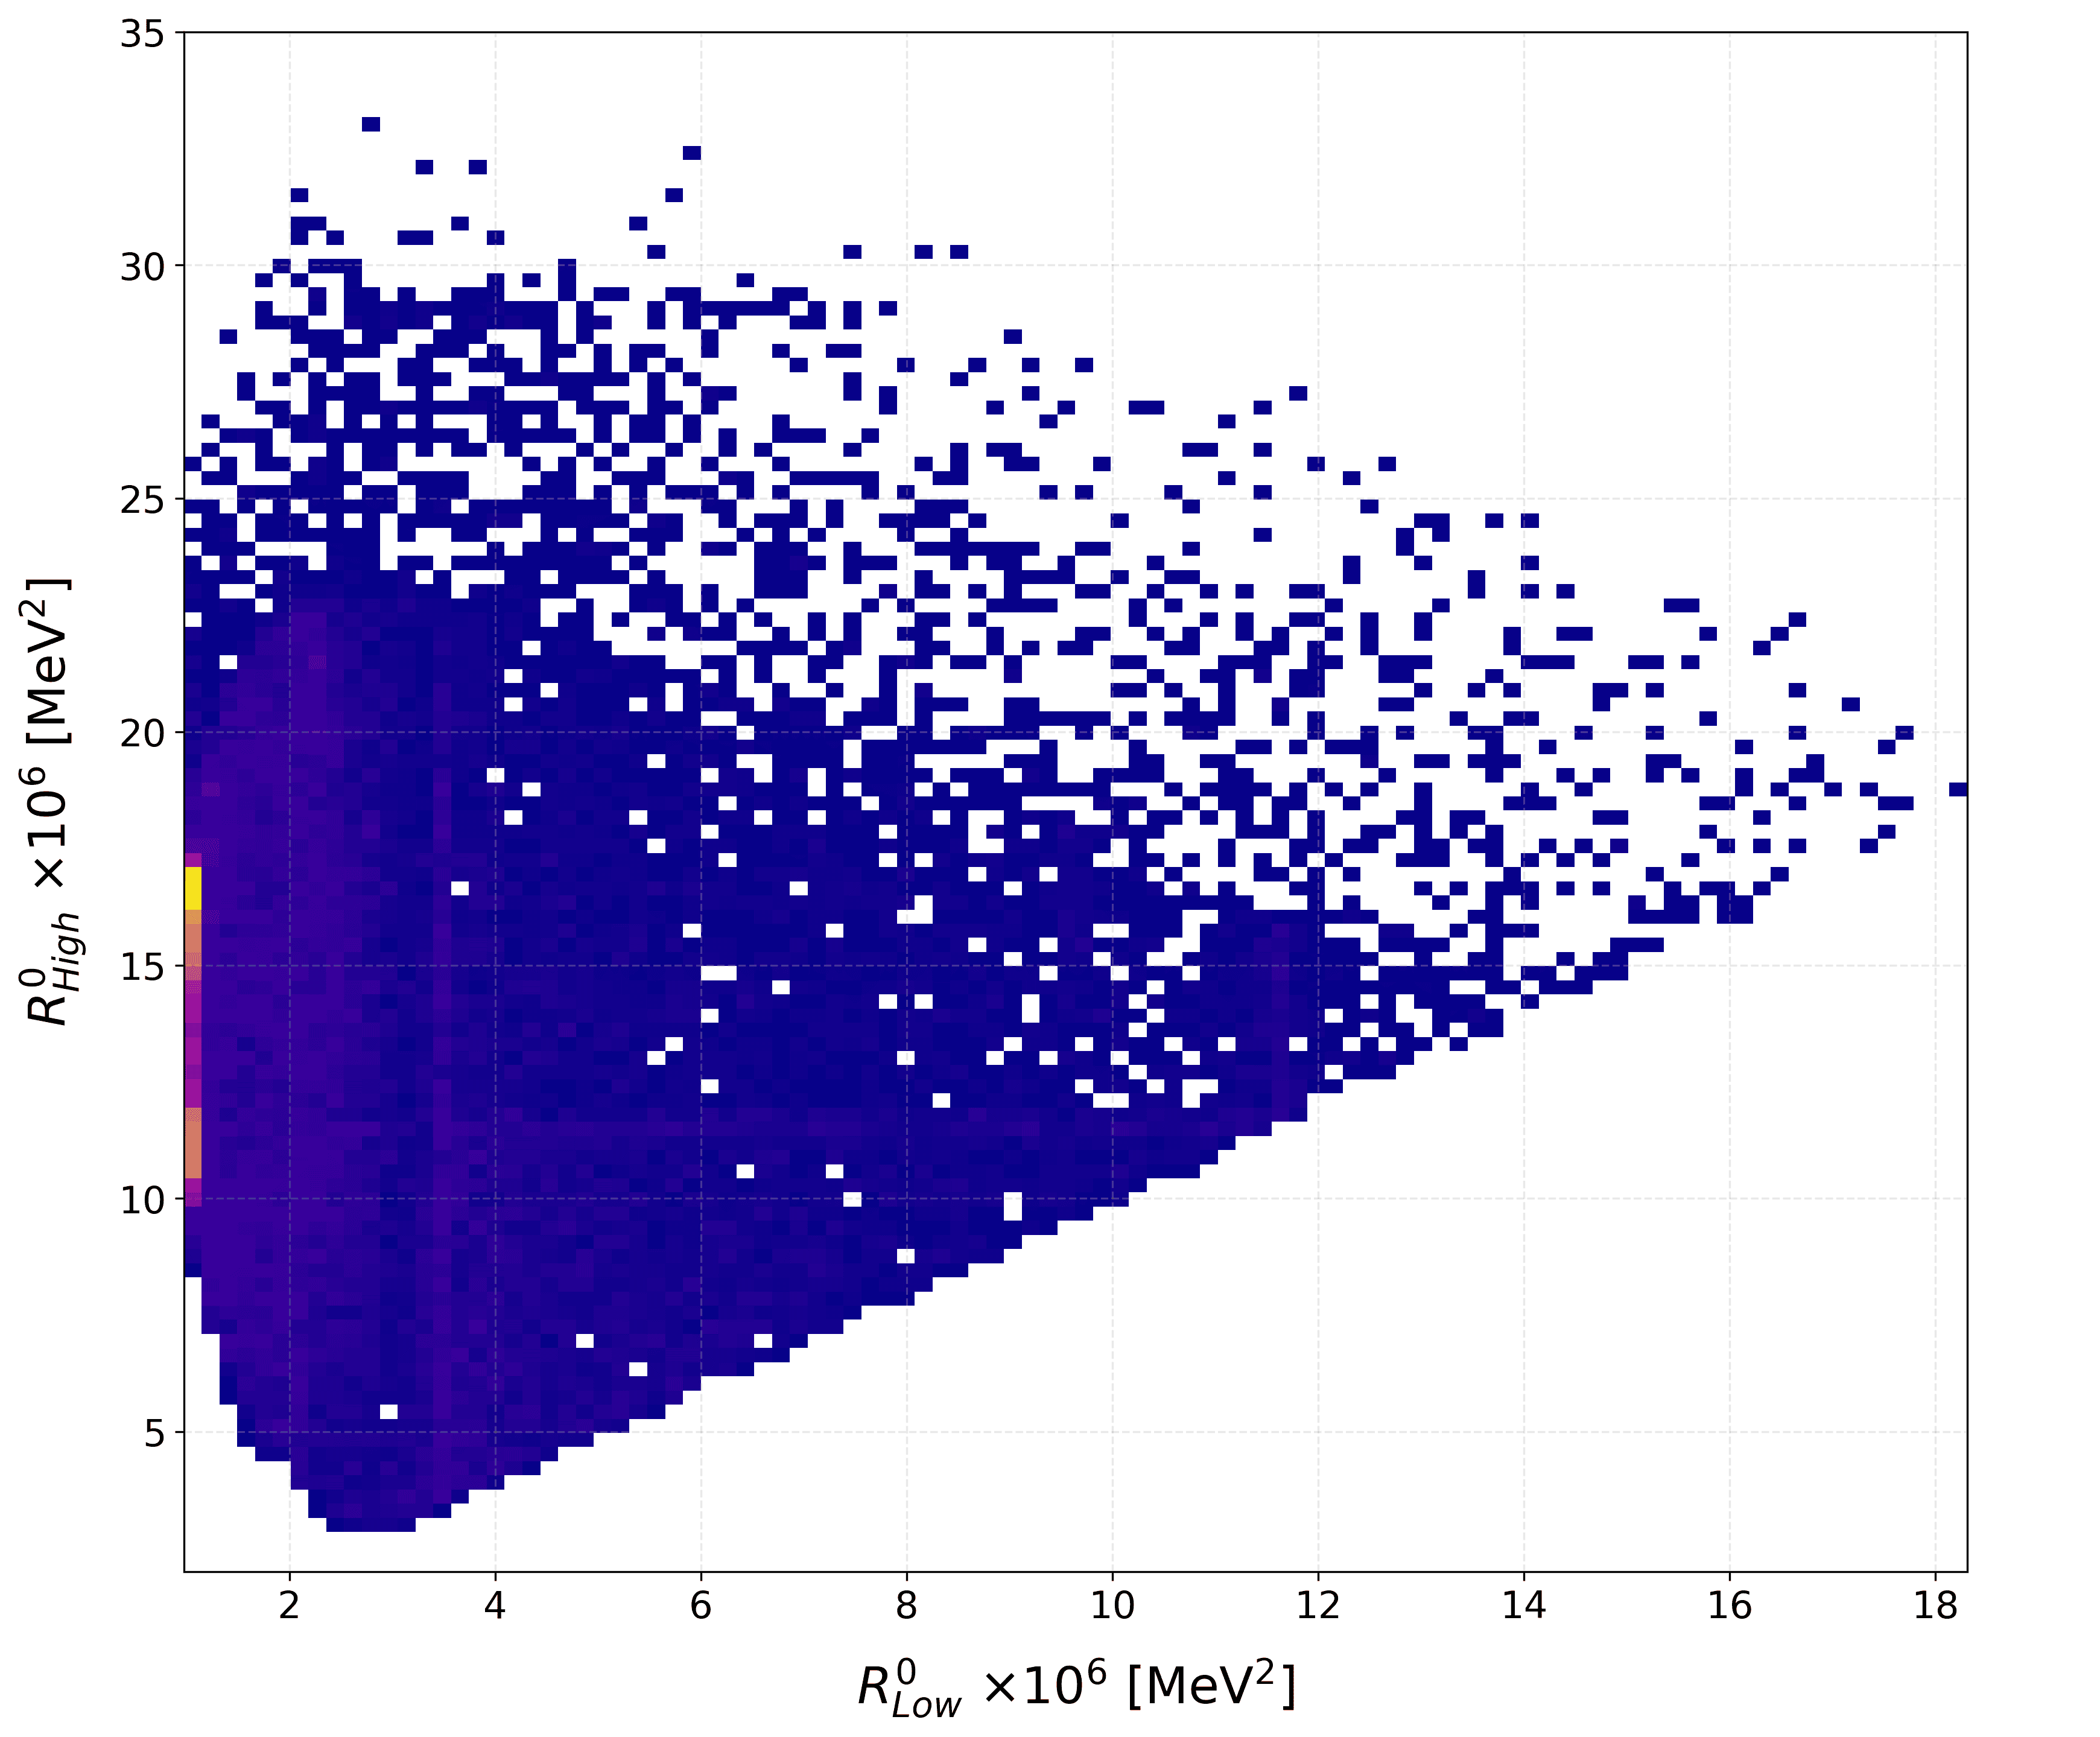
\includegraphics[width=\textwidth, scale=0.35]{Figure/hist_dalitz_data_ordering_before.png}
            \caption{Before excluding regions corresponding to the \(D^0\) and \(\chi_{c0}\) mesons.}
        \end{subfigure}
        \hfill
        \begin{subfigure}[b]{0.48\textwidth}
            \centering
            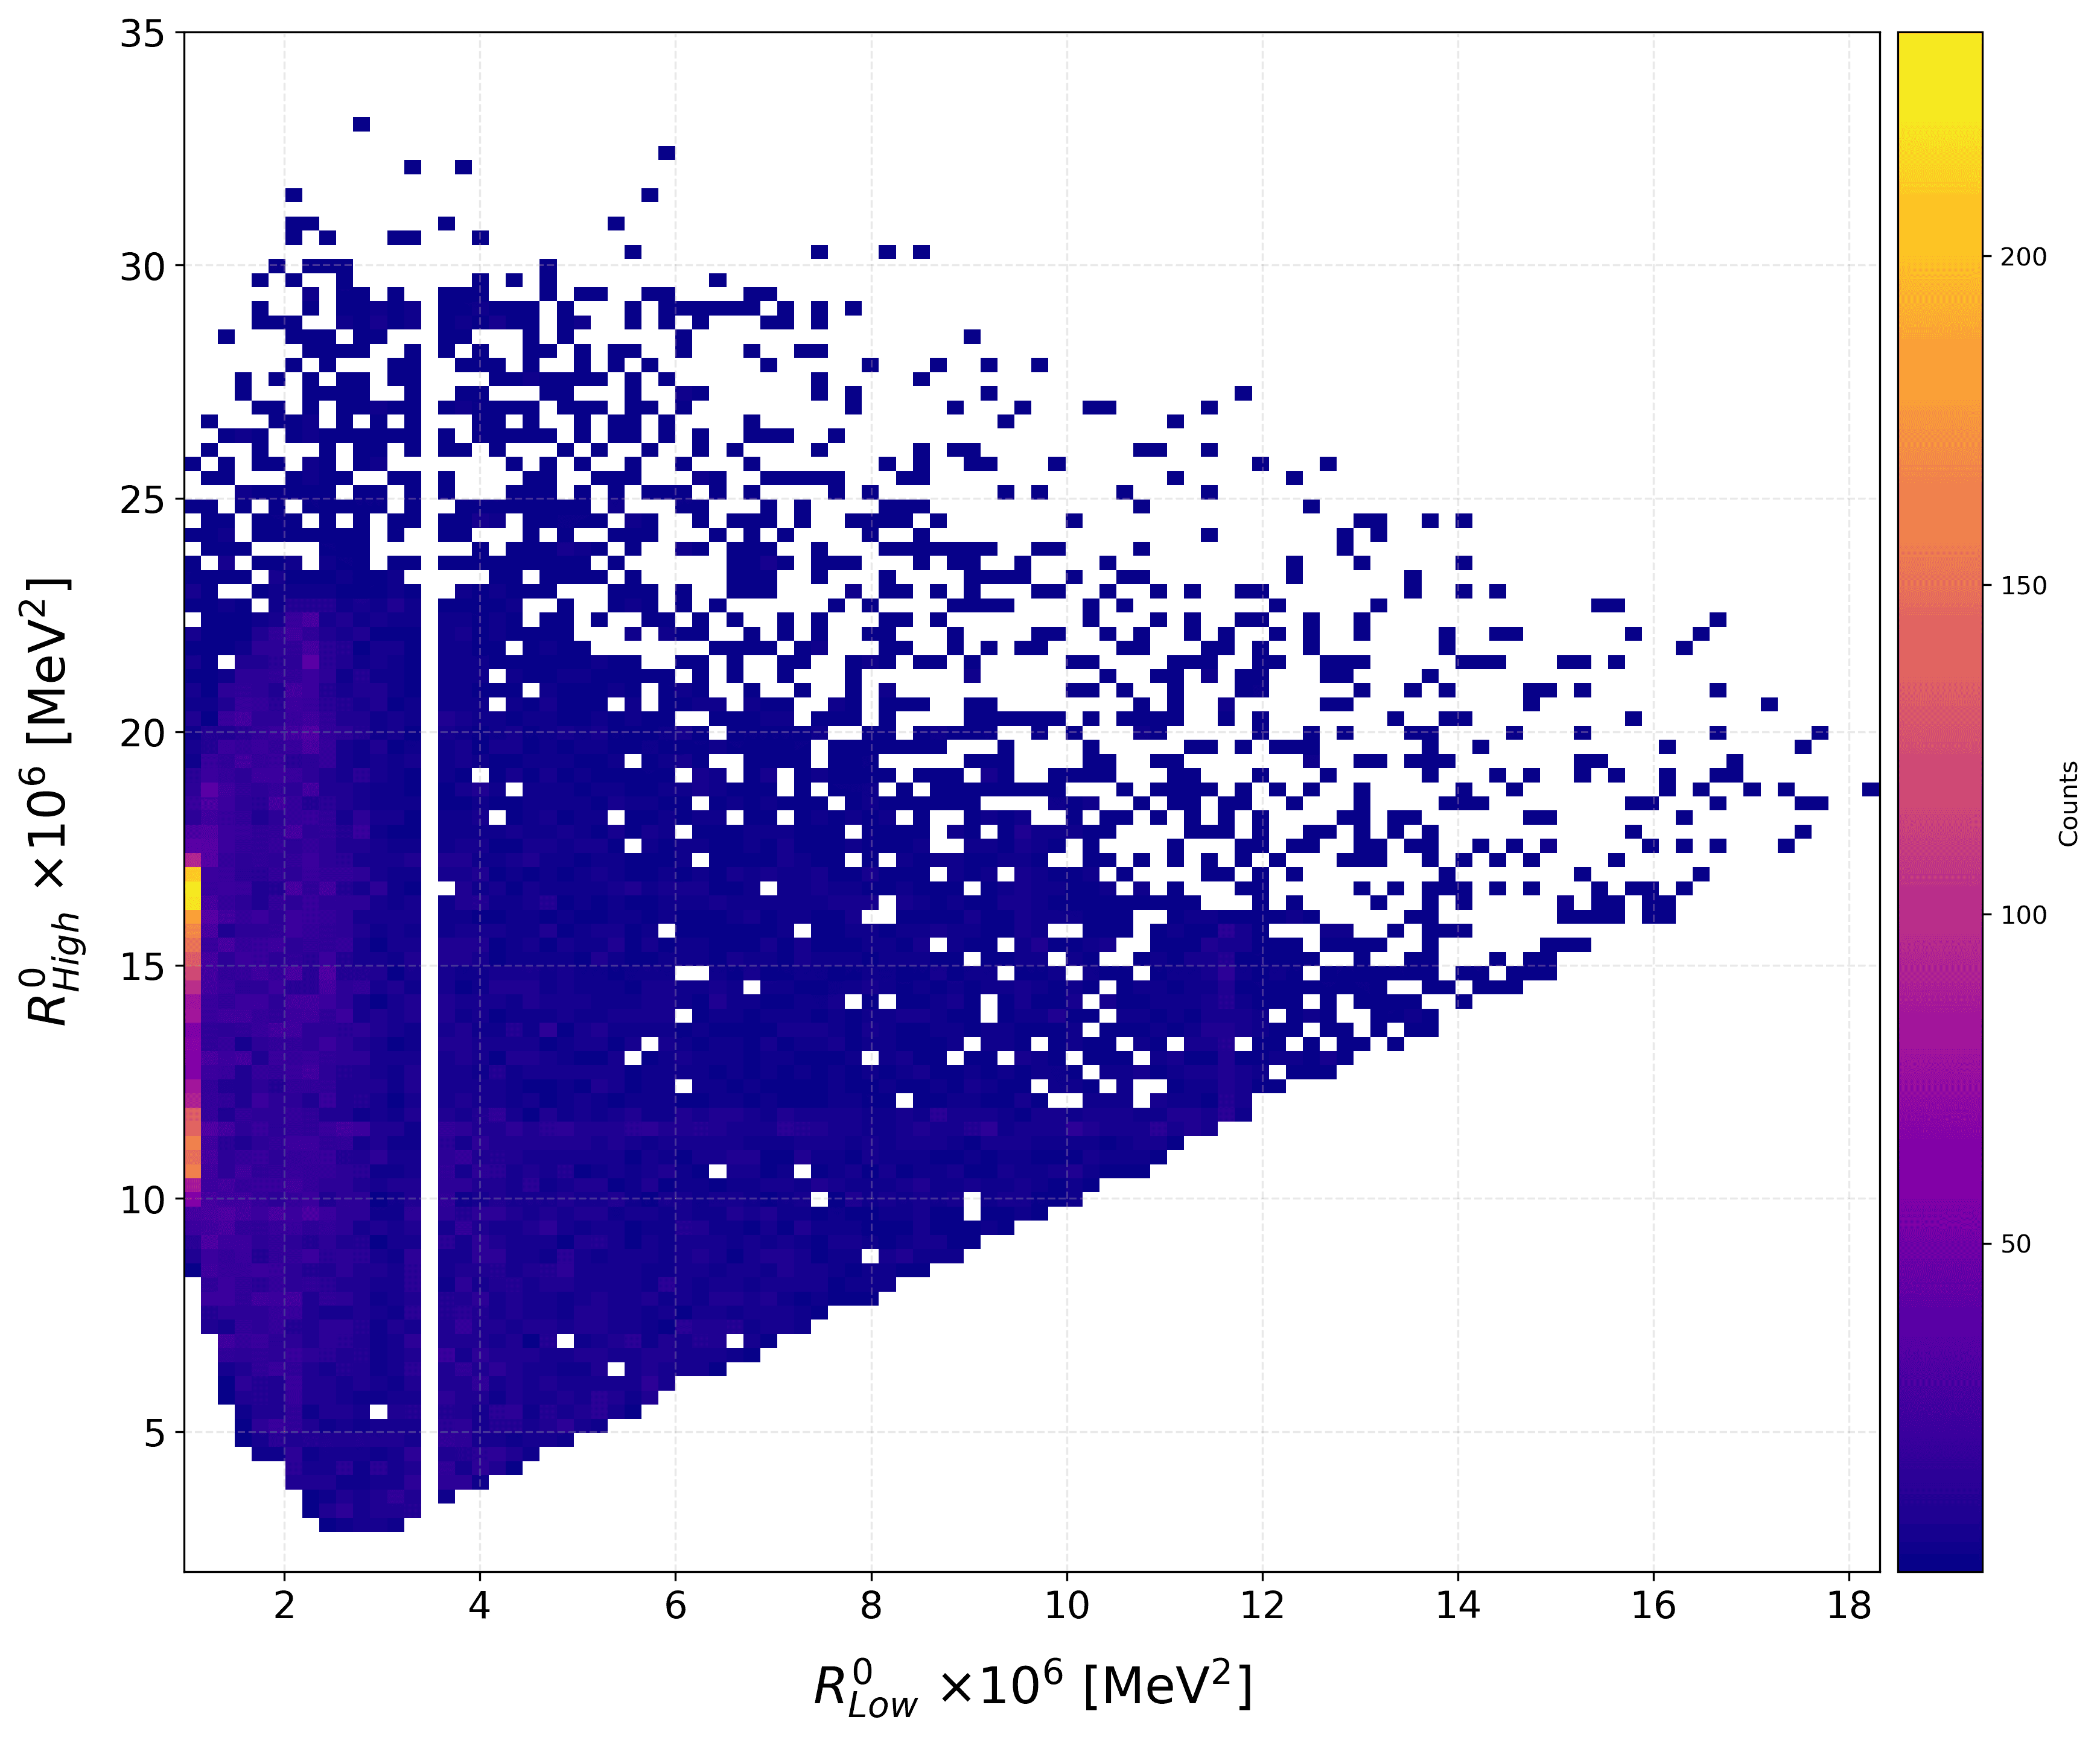
\includegraphics[width=\textwidth, scale=0.35]{Figure/hist_dalitz_data_ordering_after.png}
           \caption{After applying the cuts to remove contributions from \(D^0\) and \(\chi_{c0}\) resonances.}
        \end{subfigure}
        \caption{Dalitz plots of the \(B^\pm \to K^\pm K^\pm K^\mp\) candidates}
        \label{hist_dalitz_data_cut}
    \end{figure}
    \\

    Moreover, \(B^+\) and \(B^-\) candidates will be analyzed separately in the Dalitz plot to search for local CP asymmetries, as shown in Figure \ref{hist_dalitz_sep}.

    \begin{figure}[H]
        \centering
        \begin{subfigure}[b]{0.48\textwidth}
            \centering
            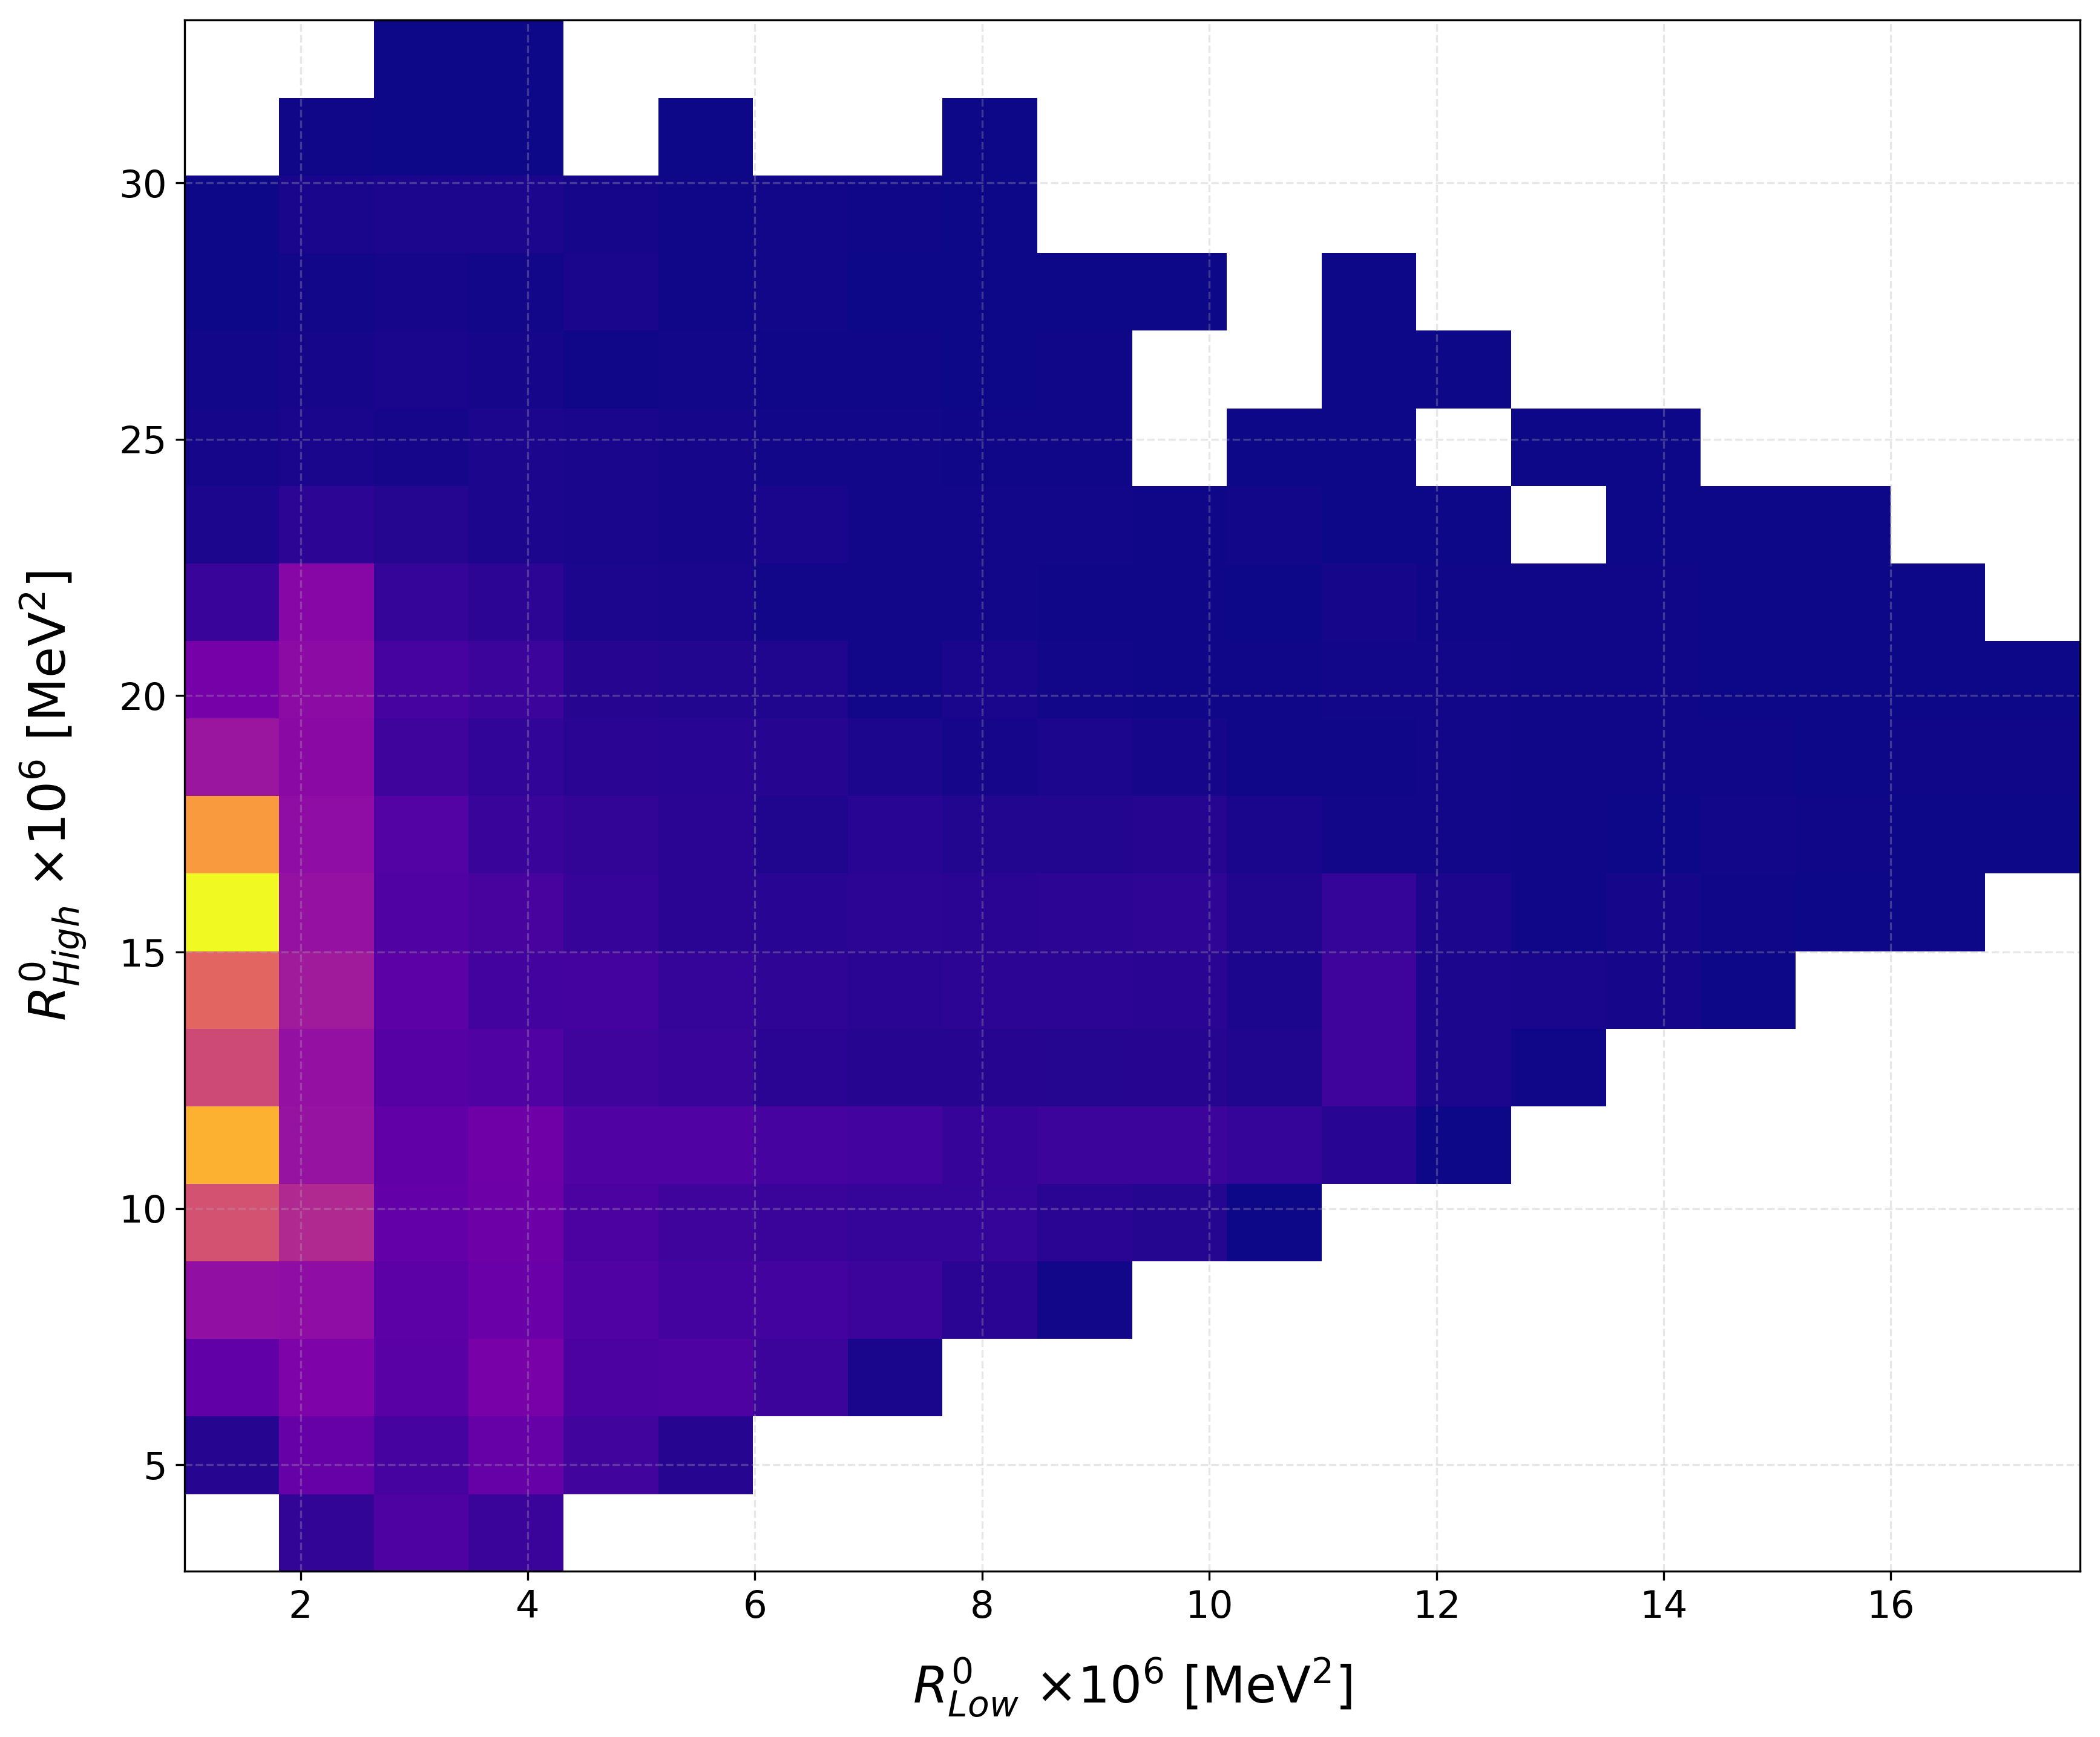
\includegraphics[width=\textwidth, scale=0.35]{Figure/hist_dalitz_plus.png}
            \caption{\(B^+\) meson}
        \end{subfigure}
        \hfill
        \begin{subfigure}[b]{0.48\textwidth}
            \centering
            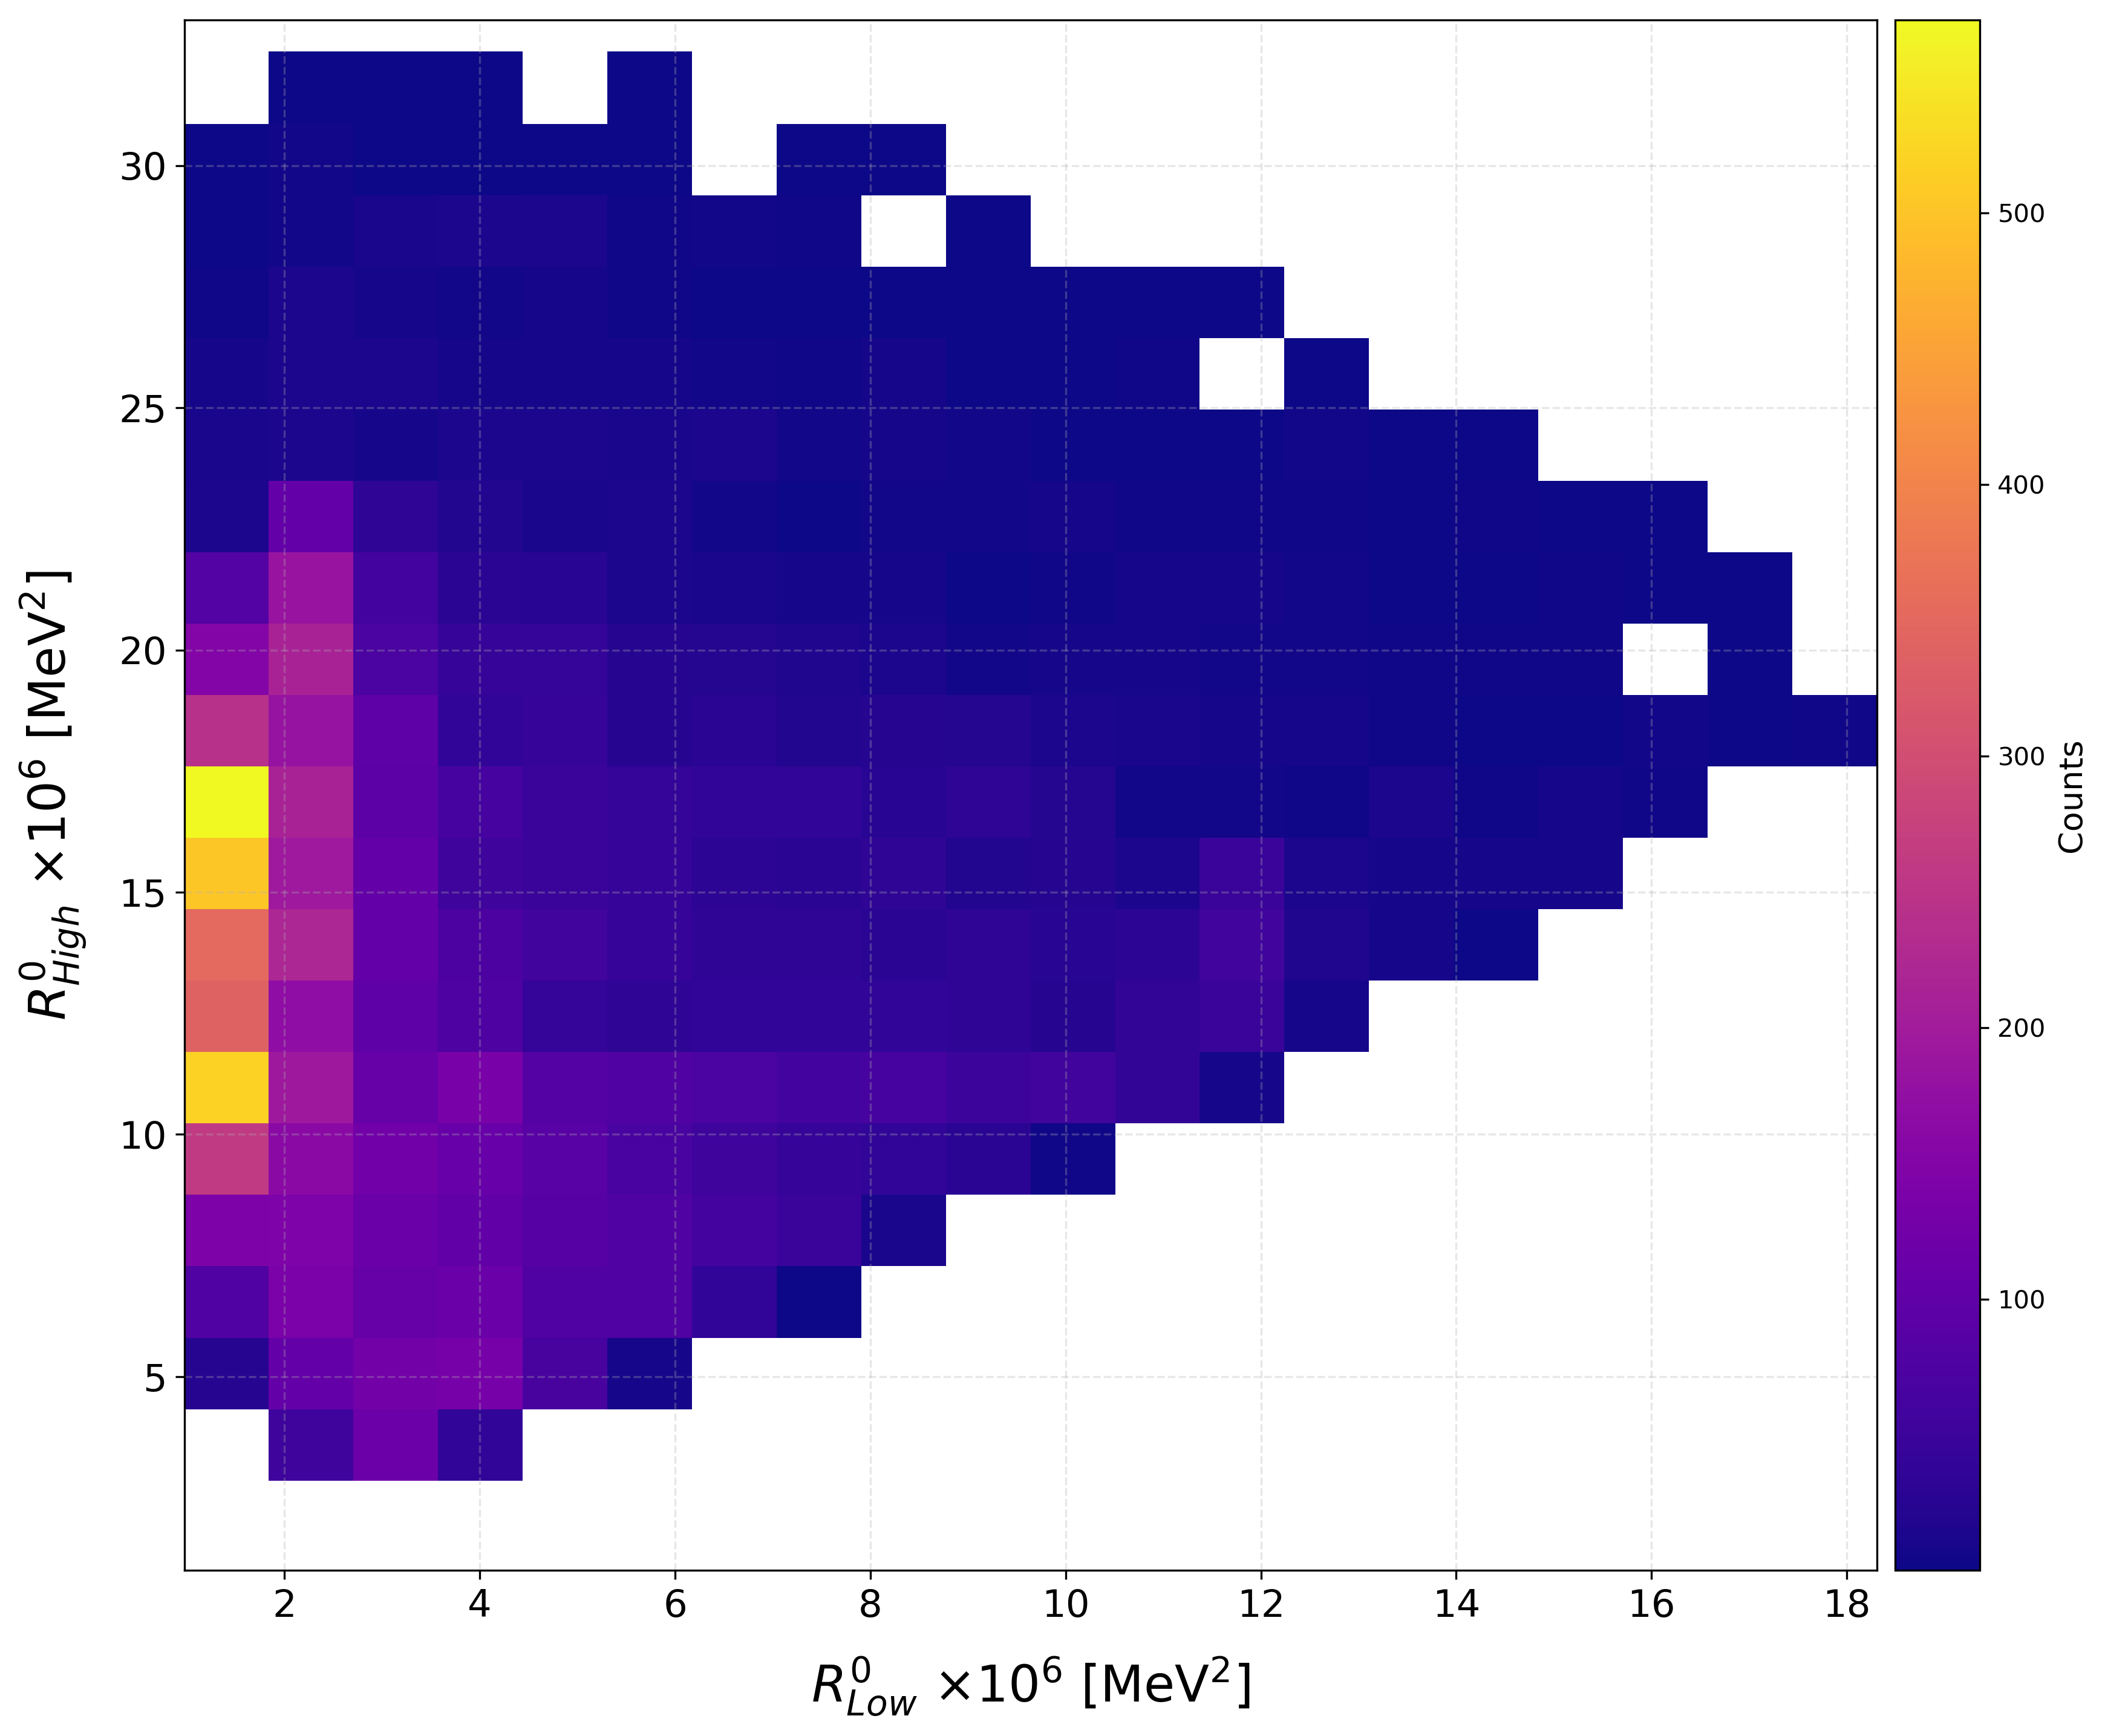
\includegraphics[width=\textwidth, scale=0.35]{Figure/hist_dalitz_minus.png}
           \caption{\(B^-\) meson}
        \end{subfigure}
        \caption{Dalitz plots of the selected \(B^+\) and \(B^-\) mesons}
        \label{hist_dalitz_sep}
    \end{figure}
    \\
    Figure \ref{hist_local} shows a clean region for observing local CP violation. Lower regions of \( R^0_{\text{Low}} \) and \( R^0_{\text{High}} \) show significant areas that are potential places to observe CP violation because these regions correspond to mass ranges where asymmetries in particle decay rates are more outstanding. Table \ref{table2} summarizes the criteria used to select the region of interest.
    \\

\begin{figure}[H]
    \centering
    \begin{subfigure}[b]{0.3\textwidth}
        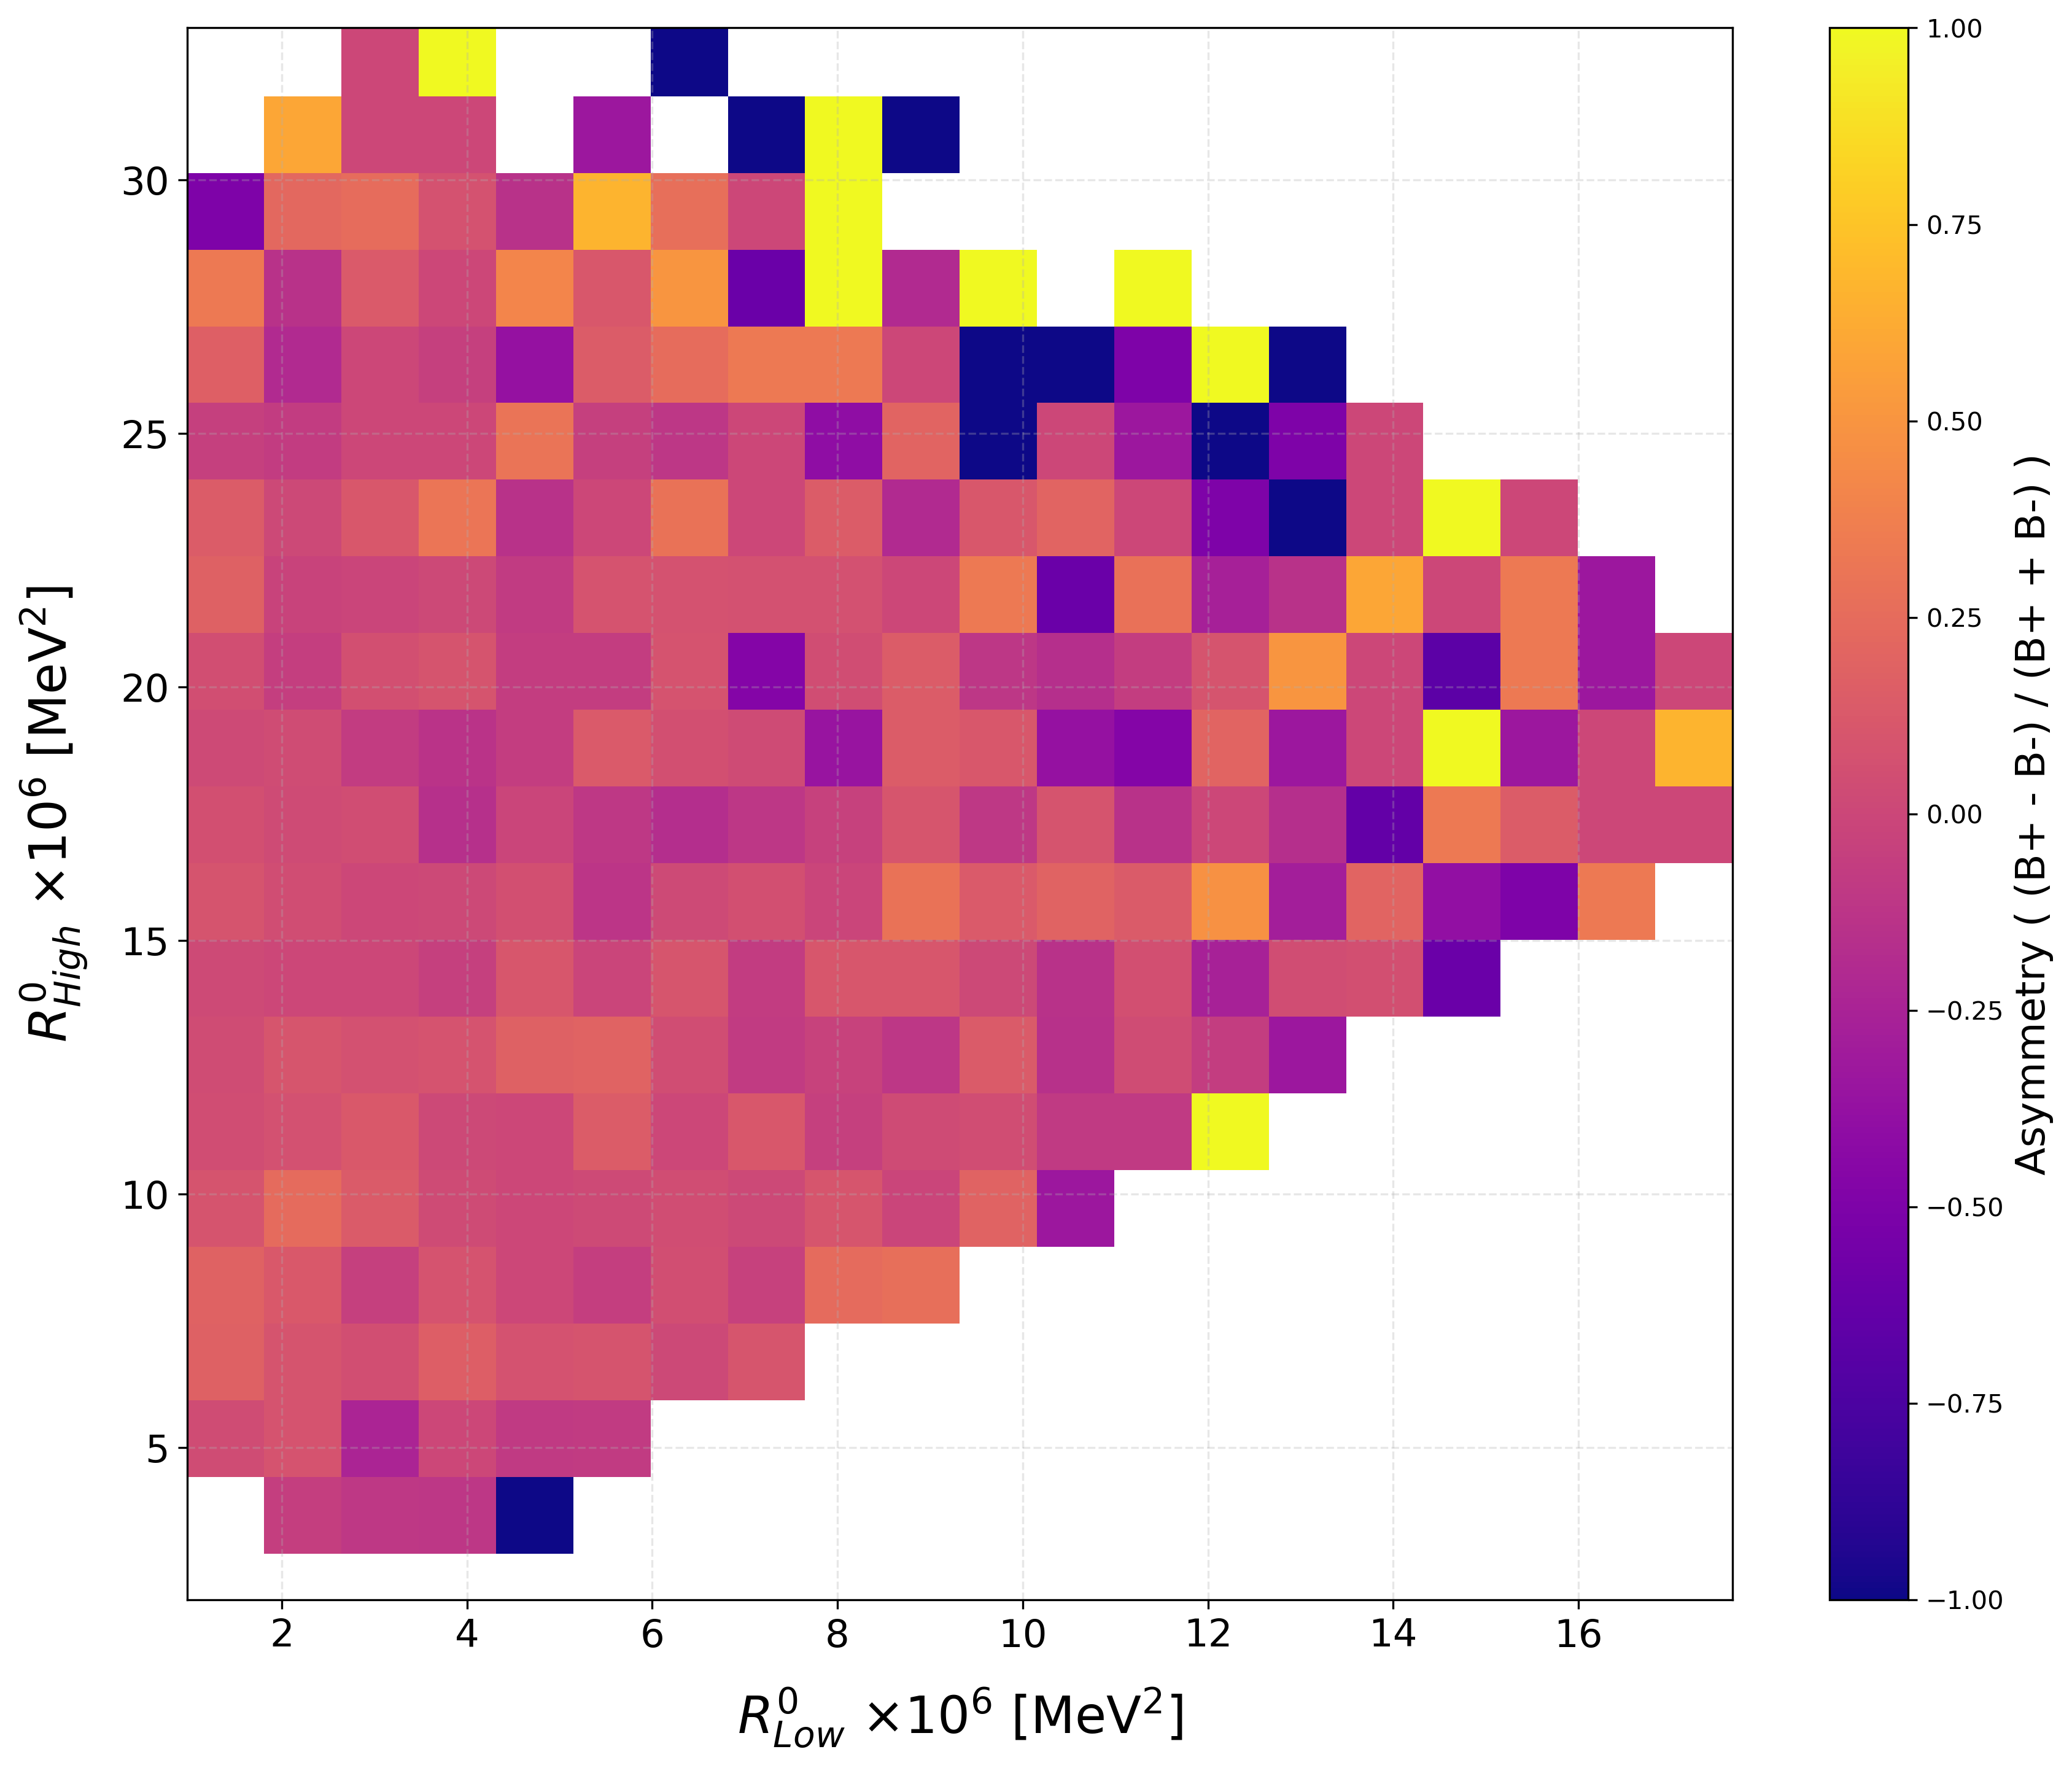
\includegraphics[width=\textwidth]{Figure/hist_dalitz_asym.png}
        \caption{Asymmetry \(A\)}
        \label{fig:dalitz_asym}
    \end{subfigure}
    \hfill
    \begin{subfigure}[b]{0.3\textwidth}
        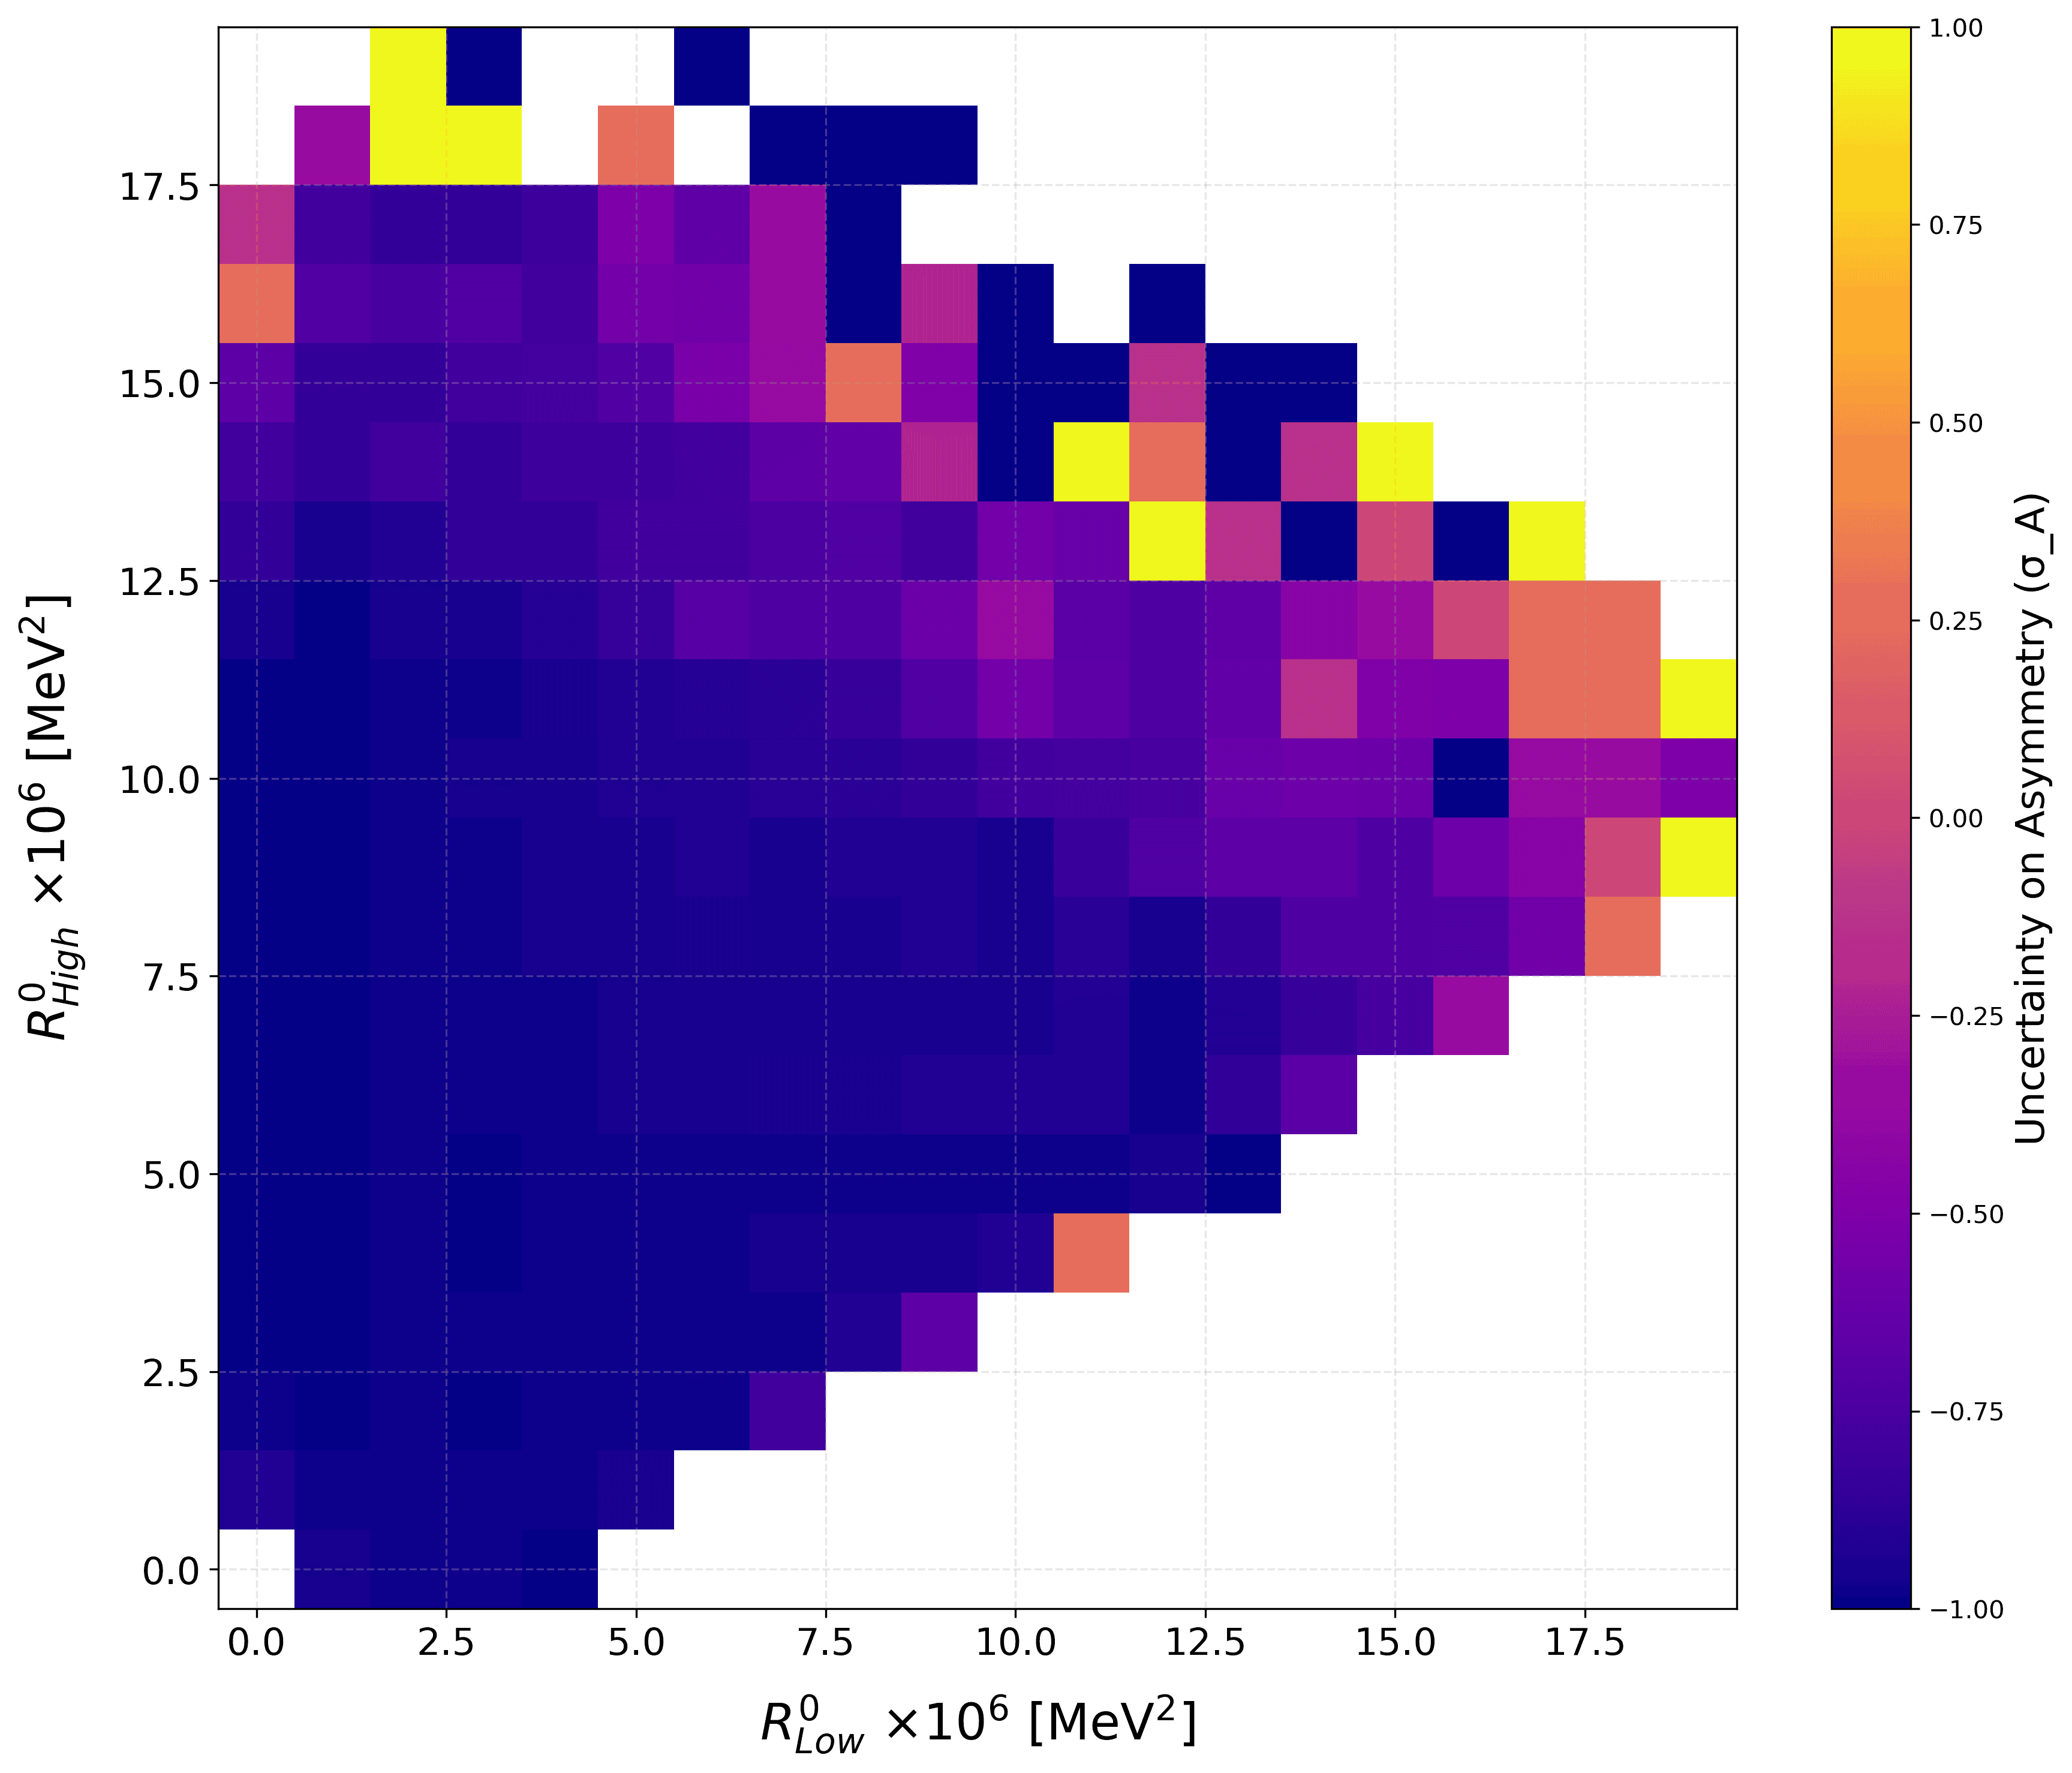
\includegraphics[width=\textwidth]{Figure/hist_dalitz_uncertainty.png}
        \caption{Statistical uncertainty \(\sigma_A\)}
        \label{fig:dalitz_uncertainty}
    \end{subfigure}
    \hfill
    \begin{subfigure}[b]{0.3\textwidth}
        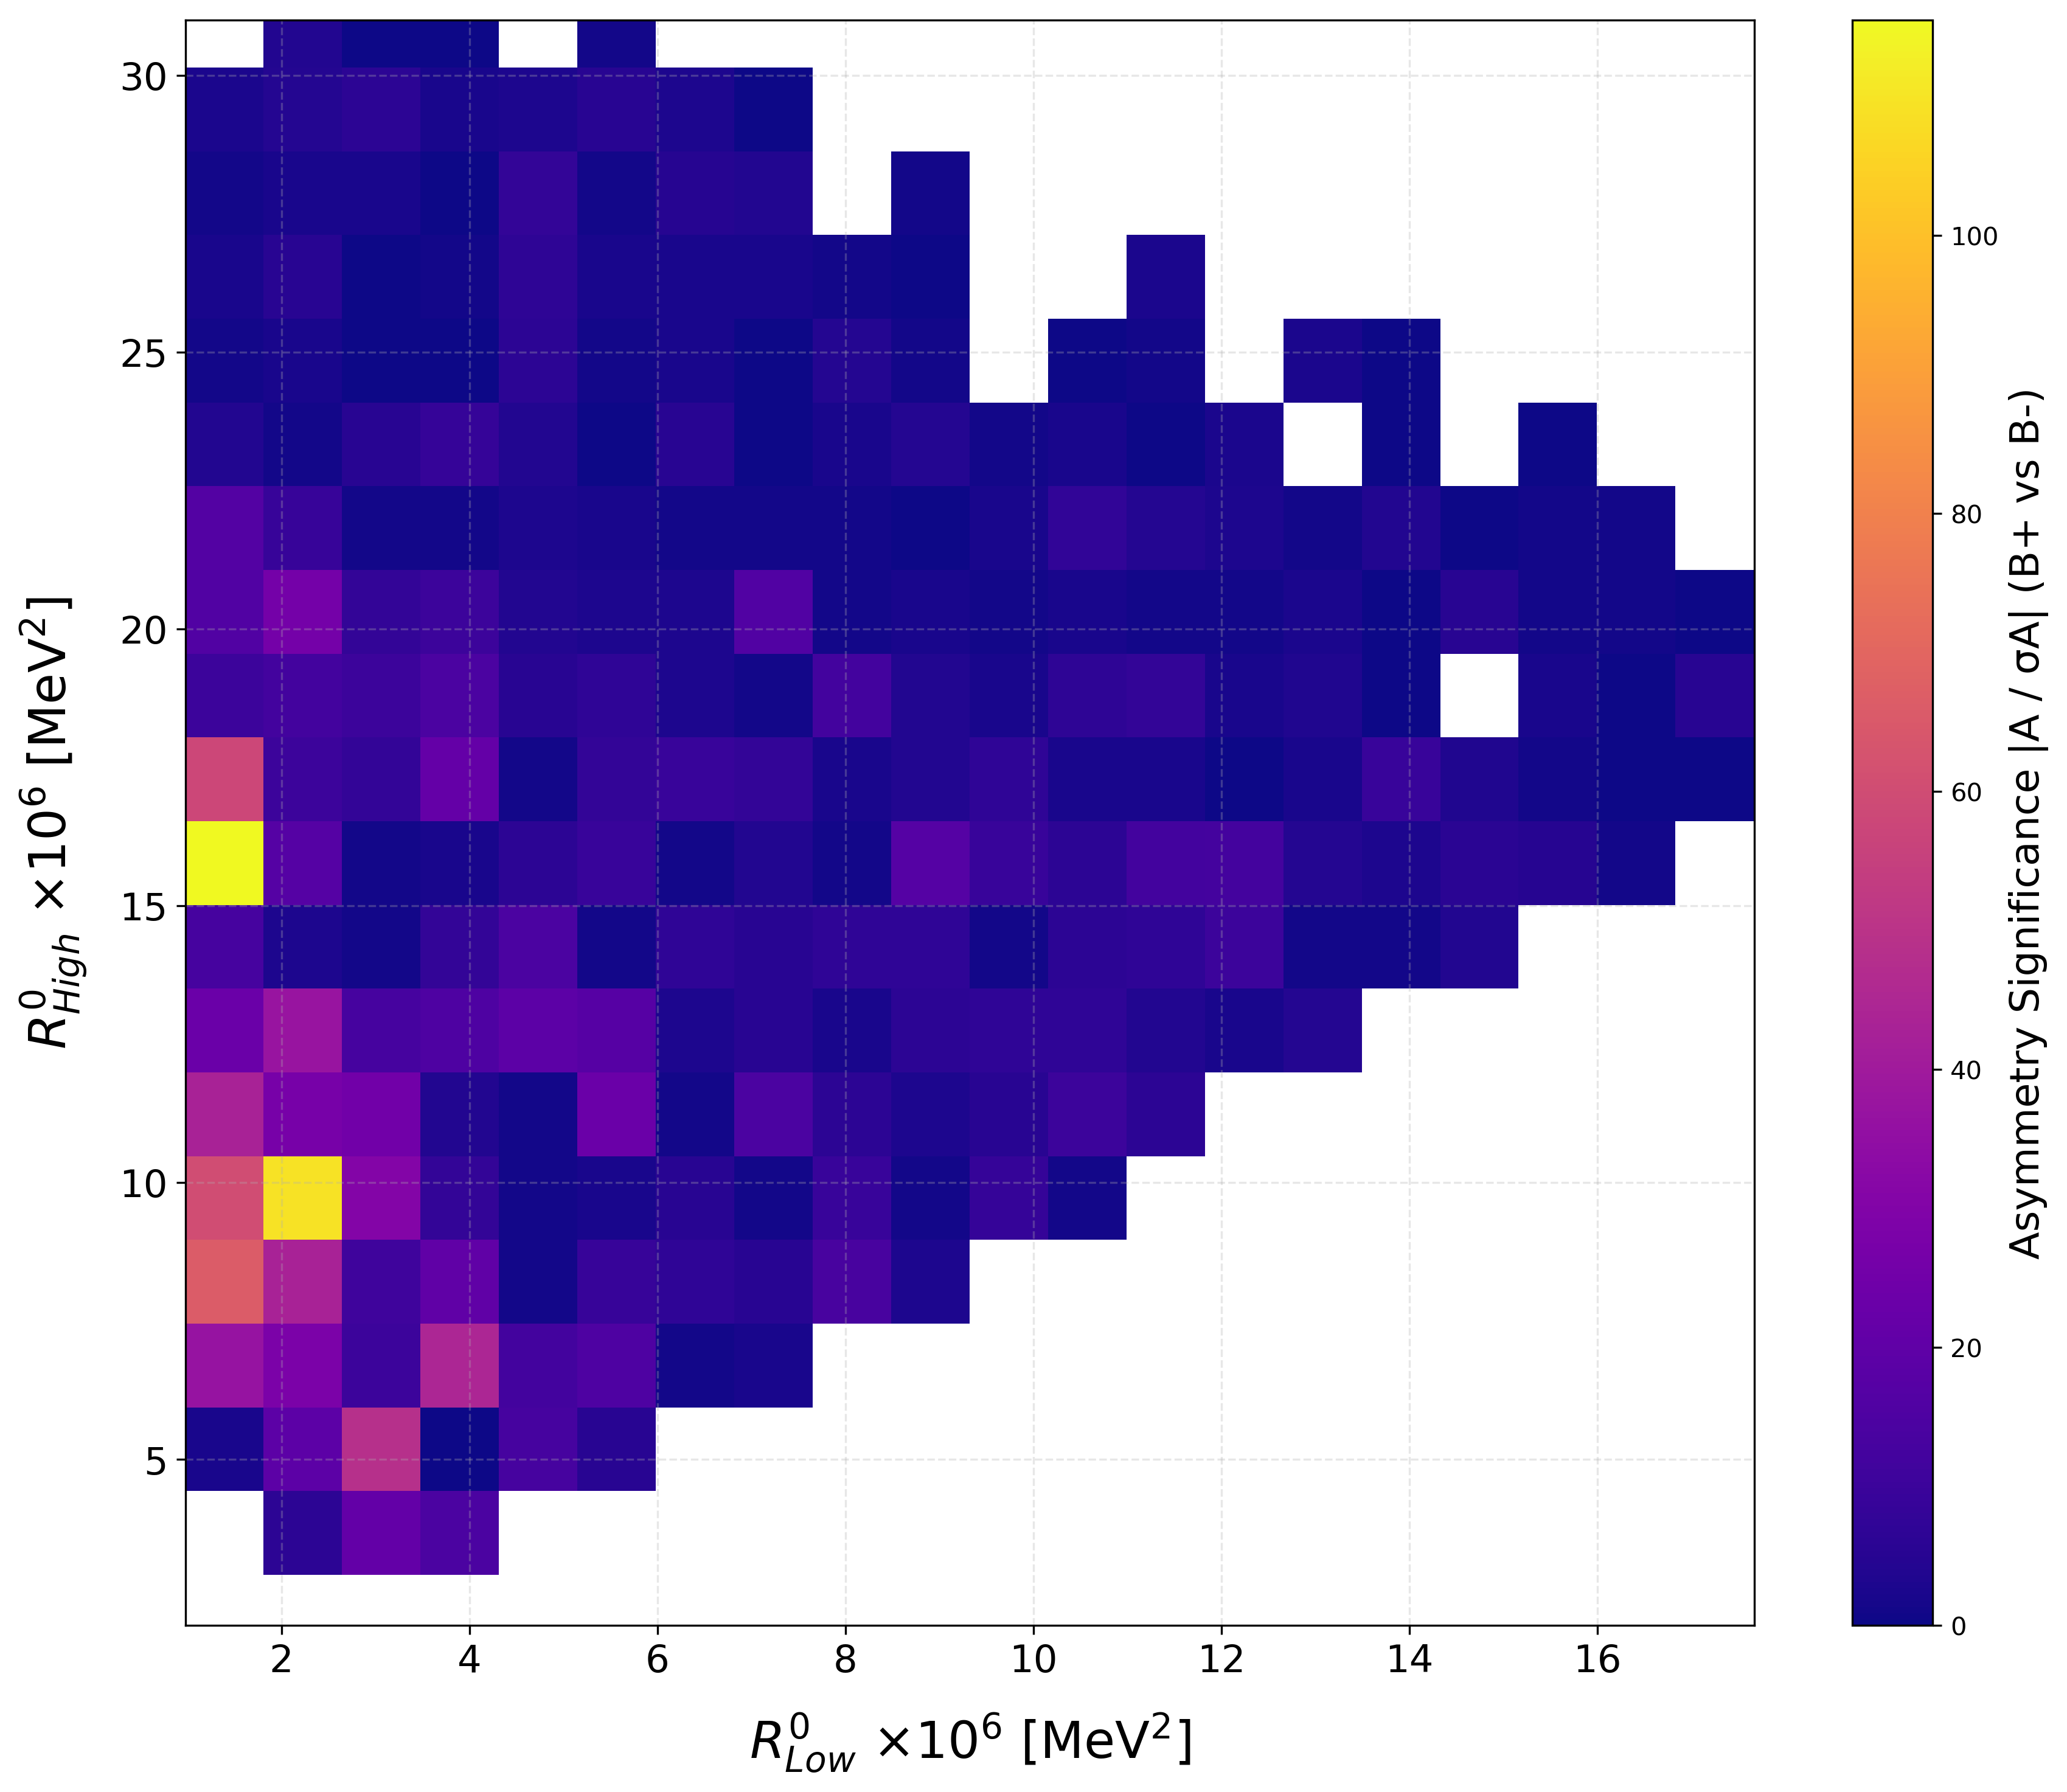
\includegraphics[width=\textwidth]{Figure/hist_dalitz_sign.png}
        \caption{Significance \(\frac{A}{\sigma_A}\)}
        \label{fig:dalitz_significance}
    \end{subfigure}
    \caption{Local CP asymmetry results showing (a) the asymmetry \(A\), (b) the statistical uncertainty \(\sigma_A\), and (c) the significance \(\frac{A}{\sigma_A}\) calculated from the Dalitz plot analysis.}
    \label{hist_local}
\end{figure}

    %% 


\begin{table}[h]
\centering
\caption{Selection criteria applied for candidate regions of local CP violation.}
\label{table2}
\begin{tabular}{ccc}
\hline
\multicolumn{3}{c}{Unit: \(10^6 \, [\mathrm{MeV}^2]\)} \\
\hline
\( R^0_{\text{Low}} < 3 \) & \text{and} \( 6 < R^0_{\text{High}} < 14 \) & \text{or} \( 15 < R^0_{\text{High}} < 16 \) \\
\hline
\end{tabular}
\end{table}



    Following the same procedure used to calculate global asymmetries in Section \ref{sec:global_asymmetry}, local CP asymmetries are evaluated by comparing event in corresponding bins of the Dalitz plots for \(B^+\) and \(B^-\) candidates. Figure \ref{hist_local} shows the asymmetry calculated using Equation \ref{asym}, the statistical uncertainty from Equation \ref{sigma} and the resulting significance according to Equation \ref{sig}. Moreover there are systematic uncertainties due to a production asymmetry between \( B^+ \) and \( B^- \) mesons as they may not be produced at the same rates. This asymmetry is estimated to be approximately 1\%. The table below shows the results obtained for local analysis.

    \begin{table}[H]
    \centering
    \begin{tabular}{lccc}
        \hline
        \textbf{Observable} & \textbf{Value} & \textbf{Uncertainty \(\sigma_A\)} & \textbf{Significance \(\frac{A}{\sigma_A}\)} \\
        \hline
        Asymmetry \(A_{local}\) & 0.1238 & 0.02085 & 6.767 \\
        \hline
    \end{tabular}
    \caption{Summary of the local CP asymmetry.}
    \label{asymmetry-results-local}
    \end{table}
    \\
    
    Therefore, the invariant mass distribution of \(B^+\) and \(B^-\) mesons can be calculated using equation \ref{eq_energy}. The plots shown in Figure~\ref{two_mass} have peaks at \( 5282.74 \pm 22.75 \, \text{MeV} \) and \( 5283.73 \pm 21.82 \, \text{MeV} \) for \( B^+ \) and \( B^- \), respectively.

    % (5283.724484879278, 21.820509390864483)
    % (5282.741932026484, 22.75673056727458)

    \begin{figure}[H]
        \centering
        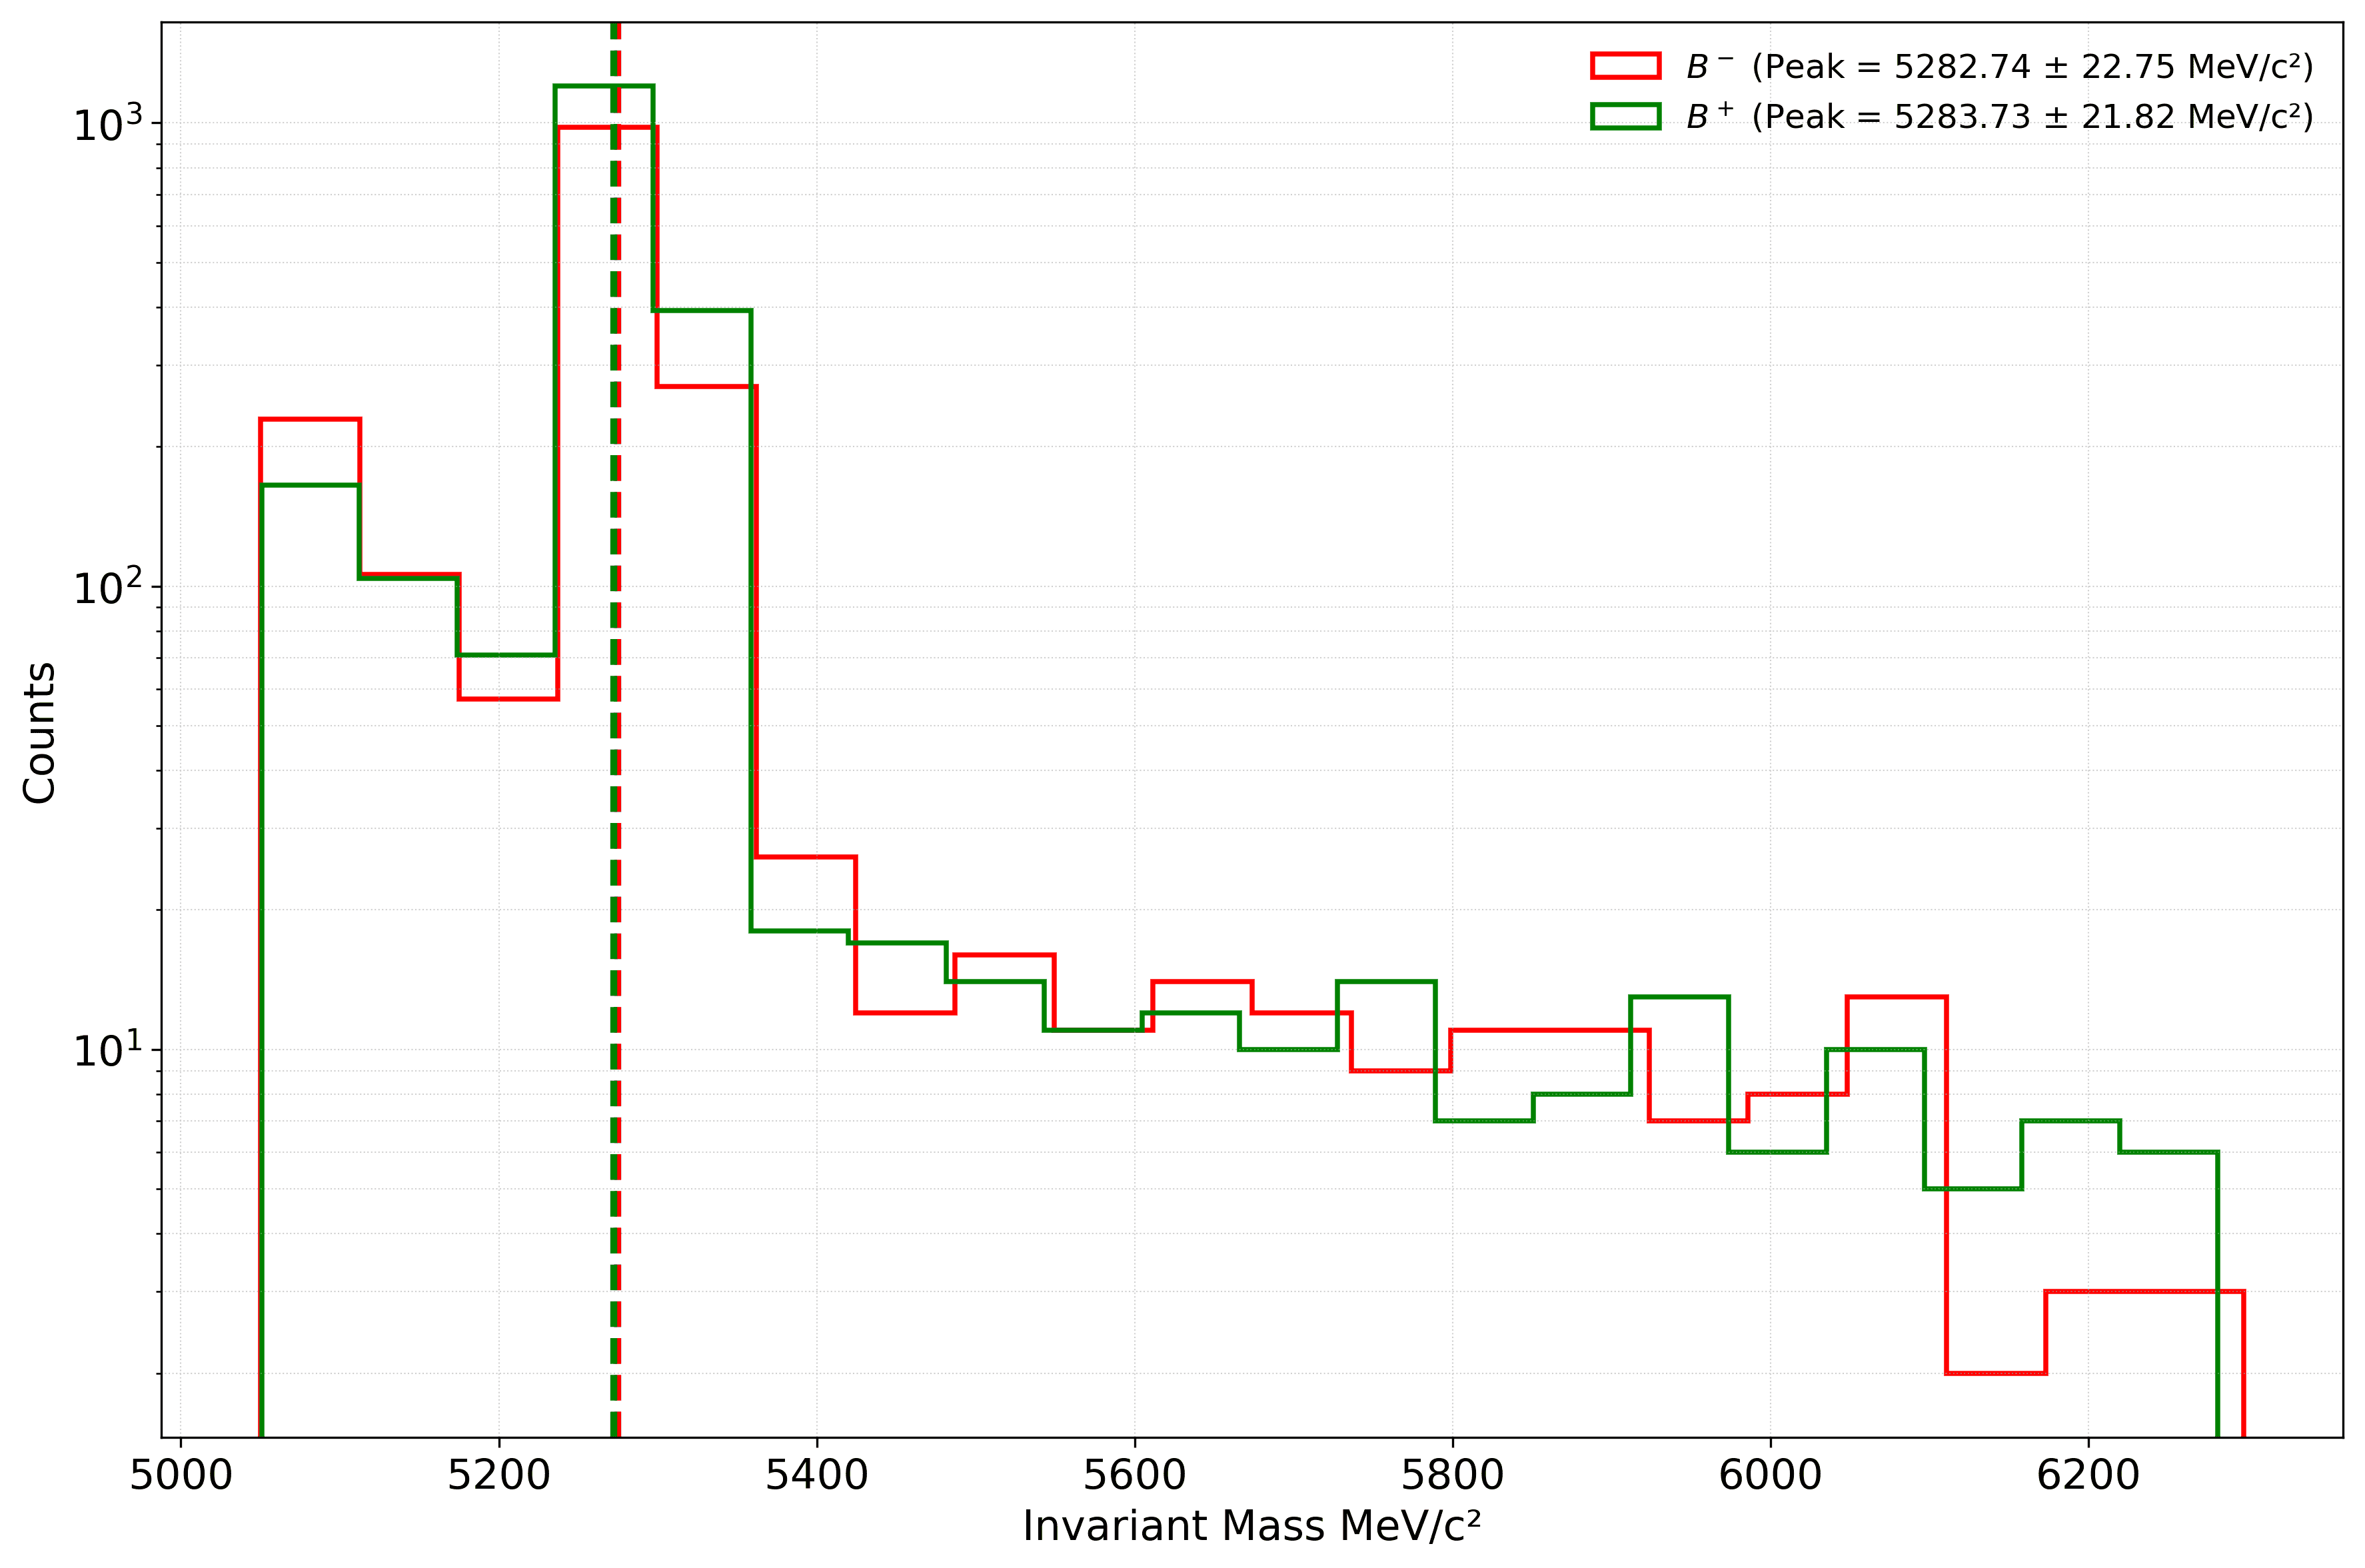
\includegraphics[scale=0.1]{Figure/hist_mass.png}
        \caption{Invariant mass distributions of the \(B^+\) and \(B^-\) mesons}
        \label{two_mass}
    \end{figure}

    